
%% bare_jrnl.tex
%% V1.4b
%% 2015/08/26
%% by Michael Shell
%% see http://www.michaelshell.org/
%% for current contact information.
%%
%% This is a skeleton file demonstrating the use of IEEEtran.cls
%% (requires IEEEtran.cls version 1.8b or later) with an IEEE
%% journal paper.
%%
%% Support sites:
%% http://www.michaelshell.org/tex/ieeetran/
%% http://www.ctan.org/pkg/ieeetran
%% and
%% http://www.ieee.org/

%%*************************************************************************
%% Legal Notice:
%% This code is offered as-is without any warranty either expressed or
%% implied; without even the implied warranty of MERCHANTABILITY or
%% FITNESS FOR A PARTICULAR PURPOSE! 
%% User assumes all risk.
%% In no event shall the IEEE or any contributor to this code be liable for
%% any damages or losses, including, but not limited to, incidental,
%% consequential, or any other damages, resulting from the use or misuse
%% of any information contained here.
%%
%% All comments are the opinions of their respective authors and are not
%% necessarily endorsed by the IEEE.
%%
%% This work is distributed under the LaTeX Project Public License (LPPL)
%% ( http://www.latex-project.org/ ) version 1.3, and may be freely used,
%% distributed and modified. A copy of the LPPL, version 1.3, is included
%% in the base LaTeX documentation of all distributions of LaTeX released
%% 2003/12/01 or later.
%% Retain all contribution notices and credits.
%% ** Modified files should be clearly indicated as such, including  **
%% ** renaming them and changing author support contact information. **
%%*************************************************************************


% *** Authors should verify (and, if needed, correct) their LaTeX system  ***
% *** with the testflow diagnostic prior to trusting their LaTeX platform ***
% *** with production work. The IEEE's font choices and paper sizes can   ***
% *** trigger bugs that do not appear when using other class files.       ***                          ***
% The testflow support page is at:
% http://www.michaelshell.org/tex/testflow/



\documentclass[journal]{IEEEtran}
%
% If IEEEtran.cls has not been installed into the LaTeX system files,
% manually specify the path to it like:
% \documentclass[journal]{../sty/IEEEtran}





% Some very useful LaTeX packages include:
% (uncomment the ones you want to load)


% *** MISC UTILITY PACKAGES ***
%
%\usepackage{ifpdf}
% Heiko Oberdiek's ifpdf.sty is very useful if you need conditional
% compilation based on whether the output is pdf or dvi.
% usage:
% \ifpdf
%   % pdf code
% \else
%   % dvi code
% \fi
% The latest version of ifpdf.sty can be obtained from:
% http://www.ctan.org/pkg/ifpdf
% Also, note that IEEEtran.cls V1.7 and later provides a builtin
% \ifCLASSINFOpdf conditional that works the same way.
% When switching from latex to pdflatex and vice-versa, the compiler may
% have to be run twice to clear warning/error messages.






% *** CITATION PACKAGES ***
%
%\usepackage{cite}
% cite.sty was written by Donald Arseneau
% V1.6 and later of IEEEtran pre-defines the format of the cite.sty package
% \cite{} output to follow that of the IEEE. Loading the cite package will
% result in citation numbers being automatically sorted and properly
% "compressed/ranged". e.g., [1], [9], [2], [7], [5], [6] without using
% cite.sty will become [1], [2], [5]--[7], [9] using cite.sty. cite.sty's
% \cite will automatically add leading space, if needed. Use cite.sty's
% noadjust option (cite.sty V3.8 and later) if you want to turn this off
% such as if a citation ever needs to be enclosed in parenthesis.
% cite.sty is already installed on most LaTeX systems. Be sure and use
% version 5.0 (2009-03-20) and later if using hyperref.sty.
% The latest version can be obtained at:
% http://www.ctan.org/pkg/cite
% The documentation is contained in the cite.sty file itself.






% *** GRAPHICS RELATED PACKAGES ***
%
\ifCLASSINFOpdf
\usepackage[pdftex]{graphicx}
% declare the path(s) where your graphic files are
%\graphicspath{{../pdf/}{../jpeg/}}
\graphicspath{{images/}}
% and their extensions so you won't have to specify these with
% every instance of \includegraphics
% \DeclareGraphicsExtensions{.pdf,.jpeg,.png}
\else
% or other class option (dvipsone, dvipdf, if not using dvips). graphicx
% will default to the driver specified in the system graphics.cfg if no
% driver is specified.
% \usepackage[dvips]{graphicx}
% declare the path(s) where your graphic files are
% \graphicspath{{../eps/}}
% and their extensions so you won't have to specify these with
% every instance of \includegraphics
% \DeclareGraphicsExtensions{.eps}
\fi
% graphicx was written by David Carlisle and Sebastian Rahtz. It is
% required if you want graphics, photos, etc. graphicx.sty is already
% installed on most LaTeX systems. The latest version and documentation
% can be obtained at: 
% http://www.ctan.org/pkg/graphicx
% Another good source of documentation is "Using Imported Graphics in
% LaTeX2e" by Keith Reckdahl which can be found at:
% http://www.ctan.org/pkg/epslatex
%
% latex, and pdflatex in dvi mode, support graphics in encapsulated
% postscript (.eps) format. pdflatex in pdf mode supports graphics
% in .pdf, .jpeg, .png and .mps (metapost) formats. Users should ensure
% that all non-photo s use a vector format (.eps, .pdf, .mps) and
% not a bitmapped formats (.jpeg, .png). The IEEE frowns on bitmapped formats
% which can result in "jaggedy"/blurry rendering of lines and letters as
% well as large increases in file sizes.
%
% You can find documentation about the pdfTeX application at:
% http://www.tug.org/applications/pdftex





% *** MATH PACKAGES ***
%
\usepackage{amsmath}
%\usepackage{calrsfs}
%\usepackage{bm}
\usepackage{amssymb}
\usepackage{array}
\usepackage{tabu}
\usepackage{float}
\usepackage{svg}
\usepackage[]{algorithm2e}
%\usepackage[colorlinks]{hyperref}
\usepackage{xcolor}

\newcolumntype{M}[1]{>{\centering\arraybackslash}m{#1}}
\newcolumntype{N}{@{}m{0pt}@{}}


\newcommand\norm[1]{\left\lVert#1\right\rVert}

\newcommand{\trans}{\mathsf{T}}






%\DeclareMathAlphabet{\pazocal}{OMS}{zplm}{m}{n}
% A popular package from the American Mathematical Society that provides
% many useful and powerful s for dealing with mathematics.
%
% Note that the amsmath package sets \interdisplaylinepenalty to 10000
% thus preventing page breaks from occurring within multiline equations. Use:
%\interdisplaylinepenalty=2500
% after loading amsmath to restore such page breaks as IEEEtran.cls normally
% does. amsmath.sty is already installed on most LaTeX systems. The latest
% version and documentation can be obtained at:
% http://www.ctan.org/pkg/amsmath






% *** SPECIALIZED LIST PACKAGES ***
%
%\usepackage{algorithmic}
% algorithmic.sty was written by Peter Williams and Rogerio Brito.
% This package provides an algorithmic environment fo describing algorithms.
% You can use the algorithmic environment in-text or within a figure
% environment to provide for a floating algorithm. Do NOT use the algorithm
% floating environment provided by algorithm.sty (by the same authors) or
% algorithm2e.sty (by Christophe Fiorio) as the IEEE does not use dedicated
% algorithm float types and packages that provide these will not provide
% correct IEEE style captions. The latest version and documentation of
% algorithmic.sty can be obtained at:
% http://www.ctan.org/pkg/algorithms
% Also of interest may be the (relatively newer and more customizable)
% algorithmicx.sty package by Szasz Janos:
% http://www.ctan.org/pkg/algorithmicx




% *** ALIGNMENT PACKAGES ***
%
%\usepackage{array}
% Frank Mittelbach's and David Carlisle's array.sty patches and improves
% the standard LaTeX2e array and tabular environments to provide better
% appearance and additional user controls. As the default LaTeX2e table
% generation code is lacking to the point of almost being broken with
% respect to the quality of the end results, all users are strongly
% advised to use an enhanced (at the very least that provided by array.sty)
% set of table tools. array.sty is already installed on most systems. The
% latest version and documentation can be obtained at:
% http://www.ctan.org/pkg/array


% IEEEtran contains the IEEEeqnarray family of commands that can be used to
% generate multiline equations as well as matrices, tables, etc., of high
% quality.




% *** SUBFIGURE PACKAGES ***
%\ifCLASSOPTIONcompsoc
%  \usepackage[caption=false,font=normalsize,labelfont=sf,textfont=sf]{subfig}
%\else
%  \usepackage[caption=false,font=footnotesize]{subfig}
%\fi
% subfig.sty, written by Steven Douglas Cochran, is the modern replacement
% for subfigure.sty, the latter of which is no longer maintained and is
% incompatible with some LaTeX packages including fixltx2e. However,
% subfig.sty requires and automatically loads Axel Sommerfeldt's caption.sty
% which will override IEEEtran.cls' handling of captions and this will result
% in non-IEEE style figure/table captions. To prevent this problem, be sure
% and invoke subfig.sty's "caption=false" package option (available since
% subfig.sty version 1.3, 2005/06/28) as this is will preserve IEEEtran.cls
% handling of captions.
% Note that the Computer Society format requires a larger sans serif font
% than the serif footnote size font used in traditional IEEE formatting
% and thus the need to invoke different subfig.sty package options depending
% on whether compsoc mode has been enabled.
%
% The latest version and documentation of subfig.sty can be obtained at:
% http://www.ctan.org/pkg/subfig




% *** FLOAT PACKAGES ***
%
%\usepackage{fixltx2e}
% fixltx2e, the successor to the earlier fix2col.sty, was written by
% Frank Mittelbach and David Carlisle. This package corrects a few problems
% in the LaTeX2e kernel, the most notable of which is that in current
% LaTeX2e releases, the ordering of single and double column floats is not
% guaranteed to be preserved. Thus, an unpatched LaTeX2e can allow a
% single column figure to be placed prior to an earlier double column
% figure.
% Be aware that LaTeX2e kernels dated 2015 and later have fixltx2e.sty's
% corrections already built into the system in which case a warning will
% be issued if an attempt is made to load fixltx2e.sty as it is no longer
% needed.
% The latest version and documentation can be found at:
% http://www.ctan.org/pkg/fixltx2e


%\usepackage{stfloats}
% stfloats.sty was written by Sigitas Tolusis. This package gives LaTeX2e
% the ability to do double column floats at the bottom of the page as well
% as the top. (e.g., "\begin{figure*}[!b]" is not normally possible in
% LaTeX2e). It also provides a command:
%\fnbelowfloat
% to enable the placement of footnotes below bottom floats (the standard
% LaTeX2e kernel puts them above bottom floats). This is an invasive package
% which rewrites many portions of the LaTeX2e float routines. It may not work
% with other packages that modify the LaTeX2e float routines. The latest
% version and documentation can be obtained at:
% http://www.ctan.org/pkg/stfloats
% Do not use the stfloats baselinefloat ability as the IEEE does not allow
% \baselineskip to stretch. Authors submitting work to the IEEE should note
% that the IEEE rarely uses double column equations and that authors should try
% to avoid such use. Do not be tempted to use the cuted.sty or midfloat.sty
% packages (also by Sigitas Tolusis) as the IEEE does not format its papers in
% such ways.
% Do not attempt to use stfloats with fixltx2e as they are incompatible.
% Instead, use Morten Hogholm'a dblfloatfix which combines the features
% of both fixltx2e and stfloats:
%
% \usepackage{dblfloatfix}
% The latest version can be found at:
% http://www.ctan.org/pkg/dblfloatfix




%\ifCLASSOPTIONcaptionsoff
%  \usepackage[nomarkers]{endfloat}
% \let\MYoriglatexcaption\caption
% \renewcommand{\caption}[2][\relax]{\MYoriglatexcaption[#2]{#2}}
%\fi
% endfloat.sty was written by James Darrell McCauley, Jeff Goldberg and 
% Axel Sommerfeldt. This package may be useful when used in conjunction with 
% IEEEtran.cls'  captionsoff option. Some IEEE journals/societies require that
% submissions have lists of figures/tables at the end of the paper and that
% figures/tables without any captions are placed on a page by themselves at
% the end of the document. If needed, the draftcls IEEEtran class option or
% \CLASSINPUTbaselinestretch interface can be used to increase the line
% spacing as well. Be sure and use the nomarkers option of endfloat to
% prevent endfloat from "marking" where the figures would have been placed
% in the text. The two hack lines of code above are a slight modification of
% that suggested by in the endfloat docs (section 8.4.1) to ensure that
% the full captions always appear in the list of figures/tables - even if
% the user used the short optional argument of \caption[]{}.
% IEEE papers do not typically make use of \caption[]'s optional argument,
% so this should not be an issue. A similar trick can be used to disable
% captions of packages such as subfig.sty that lack options to turn off
% the subcaptions:
% For subfig.sty:
% \let\MYorigsubfloat\subfloat
% \renewcommand{\subfloat}[2][\relax]{\MYorigsubfloat[]{#2}}
% However, the above trick will not work if both optional arguments of
% the \subfloat command are used. Furthermore, there needs to be a
% description of each subfigure *somewhere* and endfloat does not add
% subfigure captions to its list of figures. Thus, the best approach is to
% avoid the use of subfigure captions (many IEEE journals avoid them anyway)
% and instead reference/explain all the subfigures within the main caption.
% The latest version of endfloat.sty and its documentation can obtained at:
% http://www.ctan.org/pkg/endfloat
%
% The IEEEtran \ifCLASSOPTIONcaptionsoff conditional can also be used
% later in the document, say, to conditionally put the References on a 
% page by themselves.




% *** PDF, URL AND HYPERLINK PACKAGES ***
%
%\usepackage{url}
% url.sty was written by Donald Arseneau. It provides better support for
% handling and breaking URLs. url.sty is already installed on most LaTeX
% systems. The latest version and documentation can be obtained at:
% http://www.ctan.org/pkg/url
% Basically, \url{my_url_here}.




% *** Do not adjust lengths that control margins, column widths, etc. ***
% *** Do not use packages that alter fonts (such as pslatex).         ***
% There should be no need to do such things with IEEEtran.cls V1.6 and later.
% (Unless specifically asked to do so by the journal or conference you plan
% to submit to, of course. )


% correct bad hyphenation here
\hyphenation{op-tical net-works semi-conduc-tor}

\begin{document}
	%
	% paper title
	% Titles are generally capitalized except for words such as a, an, and, as,
	% at, but, by, for, in, nor, of, on, or, the, to and up, which are usually
	% not capitalized unless they are the first or last word of the title.
	% Linebreaks \\ can be used within to get better formatting as desired.
	% Do not put math or special symbols in the title.
	%\title{Bare Demo of IEEEtran.cls\\ for IEEE Journals}
	%
	\title{Multi-way Feature Extraction and Selection for  Alzheimer’s Disease Early Detection } 
	%
	% author names and IEEE memberships
	% note positions of commas and nonbreaking spaces ( ~ ) LaTeX will not break
	% a structure at a ~ so this keeps an author's name from being broken across
	% two lines.
	% use \thanks{} to gain access to the first footnote area
	% a separate \thanks must be used for each paragraph as LaTeX2e's \thanks
	% was not built to handle multiple paragraphs
	%
	
	\author{AA ~AA,
		AA~AA% <-this % stops a space
		\thanks{M. Shell was with the Department
			of Electrical and Computer Engineering, Georgia Institute of Technology, Atlanta,
			GA, 30332 USA e-mail: (see http://www.michaelshell.org/contact.html).}% <-this % stops a space
		\thanks{J. Doe and J. Doe are with Anonymous University.}% <-this % stops a space
		\thanks{Manuscript received April 19, 2005; revised August 26, 2015.}}
	
	% note the % following the last \IEEEmembership and also \thanks - 
	% these prevent an unwanted space from occurring between the last author name
	% and the end of the author line. i.e., if you had this:
	% 
	% \author{....lastname \thanks{...} \thanks{...} }
	%                     ^------------^------------^----Do not want these spaces!
	%
	% a space would be appended to the last name and could cause every name on that
	% line to be shifted left slightly. This is one of those "LaTeX things". For
	% instance, "\textbf{A} \textbf{B}" will typeset as "A B" not "AB". To get
	% "AB" then you have to do: "\textbf{A}\textbf{B}"
	% \thanks is no different in this regard, so shield the last } of each \thanks
	% that ends a line with a % and do not let a space in before the next \thanks.
	% Spaces after \IEEEmembership other than the last one are OK (and needed) as
	% you are supposed to have spaces between the names. For what it is worth,
	% this is a minor point as most people would not even notice if the said evil
	% space somehow managed to creep in.
	
	
	
	% The paper headers
	\markboth{Journal of \LaTeX\ Class Files,~Vol.~14, No.~8, August~2015}%
	{Shell \MakeLowercase{\textit{et al.}}: Bare Demo of IEEEtran.cls for IEEE Journals}
	% The only time the second header will appear is for the odd numbered pages
	% after the title page when using the twoside option.
	% 
	% *** Note that you probably will NOT want to include the author's ***
	% *** name in the headers of peer review papers.                   ***
	% You can use \ifCLASSOPTIONpeerreview for conditional compilation here if
	% you desire.
	
	
	
	
	% If you want to put a publisher's ID mark on the page you can do it like
	% this:
	%\IEEEpubid{0000--0000/00\$00.00~\copyright~2015 IEEE}
	% Remember, if you use this you must call \IEEEpubidadjcol in the second
	% column for its text to clear the IEEEpubid mark.
	
	
	
	% use for special paper notices
	%\IEEEspecialpapernotice{(Invited Paper)}
	
	
	
	
	% make the title area
	\maketitle
	
	% As a general rule, do not put math, special symbols or citations
	% in the abstract or keywords.
	\begin{abstract}
		Recently machine learning methods had gain lots of publicity among researchers in order to analyze the brain images such as functional Magnetic Resonance Imaging(fMRI) to obtain better understanding of the brain and brain related disease such as Alzheimer's disease. Classification methods has been deployed in order to discriminate Alzheimer's disease from normal controls. The majority of deployed techniques rely on constructing the functional connectivity (FC) and use the vectorized FC as the input for the classifiers which has two main drawbacks 1) The need for constructing the FC 2) The loss of possible valuable structural information in the vectorization step.
		Considering these problems and based on the 4D nature of the data, we have came up with a novel framework which omits the FC construction part and preserve the structural integrity of data for the classification.
		The proposed framework uses the High Order Singular Value Decomposition (HOSVD) in order to prune the classes and select the proper basis for each of them. This framework also allows us to obtain an FC matrix based on a class but not a single sample which helps us to shed more lights on the brain abnormalities in the Alzheimers disease at its early stages. 
		Extensive experiments using the ADNI dataset demonstrate that
		our proposed framework effectively boosts the fMRI classification performance in Alzheimer's disease.
	\end{abstract}
	
	
	
	% Note that keywords are not normally used for peerreview papers.
	\begin{IEEEkeywords}
		IEEE, IEEEtran, journal, \LaTeX, paper, template.
	\end{IEEEkeywords}
	
	
	
	
	
	
	% For peer review papers, you can put extra information on the cover
	% page as needed:
	% \ifCLASSOPTIONpeerreview
	% \begin{center} \bfseries EDICS Category: 3-BBND \end{center}
	% \fi
	%
	% For peerreview papers, this IEEEtran command inserts a page break and
	% creates the second title. It will be ignored for other modes.
	\IEEEpeerreviewmaketitle
	
	
	
	\section{Introduction}
	% The very first letter is a 2 line initial drop letter followed
	% by the rest of the first word in caps.
	% 
	% form to use if the first word consists of a single letter:
	% \IEEEPARstart{A}{demo} file is ....
	% 
	% form to use if you need the single drop letter followed by
	% normal text (unknown if ever used by the IEEE):
	% \IEEEPARstart{A}{}demo file is ....
	% 
	% Some journals put the first two words in caps:
	% \IEEEPARstart{T}{his demo} file is ....
	% 
	% Here we have the typical use of a "T" for an initial drop letter
	% and "HIS" in caps to complete the first word.
	\IEEEPARstart{A}{lzheimer’s} disease (AD) is a progressive neurodegenerative disorder with a long pre-morbid asymptomatic period \cite{r01} which affects millions of elderly individuals worldwide. It is predicted that the number of affected people will double in the next 20 years, and 1 in 85 people will be affected by 2050 \cite{r02}. The predominant clinical symptoms of AD include a decline in some important brain cognitive and intellectual abilities, such as memory, thinking, and reasoning. Precise diagnosis of AD, especially at its early warning stage: early Mild Cognitive Impairment (eMCI), enables treatments to delay or even avoid such disorders \cite{r03}.  
	
	
	In recent years, brain imaging techniques like Positron Emission Tomography(PET) \cite{r21}, Electroencephalography (EEG)\cite{r22} and functional Magnetic Resonance Imaging (fMRI)\cite{r23} have been used in analysis of AD. Due to the high spatial resolution and relatively lower costs, fMRI is vastly used among researchers in order to monitor brain activities especially in AD and all it's stages in which detecting abnormalities within small brain regions is essential. 
	An fMRI sample is naturally a 4D tensor consisting of 3D voxels moving in time, and each voxel contains an intensity value that is proportional to the strength of the Blood Oxygenation Level Dependent(BOLD) signal , which is a measure of the changes in blood flow, to estimate the active regions in the brain\cite{r07}.
	Resting State fMRI(rs-fMRI) is an fMRI technique in which the patient is asked to rest(without sleeping) during the whole scan, is usually used in order to analyze the brain diseases like AD or autism. rs-fMRI focuses on the low-frequency $\left( < 0.1 Hz \right)$  oscillations of BOLD signal, which presents the underlying neuronal activation patterns of brain regions[8]–[10]. 
	
{\color{red} * * * * * * * * * * * * * * * *}

Since the number of voxels within a single full scan is high 
($5000$ up to roughly $200,000$[ref(Definingnodes)]) and they form strong spatial relations, parcellation of the brain for further analysis has moved toward the use
of anatomical atlases. These atlases are strictly defined using
anatomical features of the brain, like locations of common gyri
and do not rely on any functional information. To generate data
using an atlas based approach, the BOLD signal from all voxels is averaged within each brain region called Region of Interest(ROI).
By putting together the average time-series for all the ROIs, the $i$th volume would become $X_i \in \mathbb{R}^{T \times R} , i = \{1,2,\cdots, S\}$ in which $R$, $T$ and $S$ represents the number of ROIs, time points and samples respectively. The process of obtaining such matrix is shown in Figure \eqref{g1.1}. 
Two major studies could carry out using these  $X_i$s: 
\begin{itemize}
	\item Identifying patients with brain disorders: Because of the nature of the data, advance machine learning techniques should be deployed inorder to detect any abnormalities within an individual scan. 
	In recent years, classification techniques has been deployed  to classify the $X_i$s. These studies holds great promise for eMCI detection.     
	\item Extracting common patterns caused by a disease: An other useful information that could be extracted from such data, is the detection of common patterns emerging from a certain brain disorder such as eMCI. For example, compared with the healthy,  MCI patients have been observed both increased and decreased activities within  different brain regions [4].
\end{itemize}

A common and yet powerful tool for fMRI analysis is Functional Connectivity (FC) network.  In
functional brain networks, nodes represent ROIs, and edges measure functional connectivity
between pairs of nodes. Functional connectivity is an observable
phenomenon quantifiable with measures of statistical dependencies, such as correlations, coherence, or transfer entropy([][]). FC is simply a $region \times region$ matrix $\bar{X}_i$ in which $\bar{x_{ij}}$ represents the functional connectivity between the $i$th and $j$th ROI. Recent studies have shown that some brain disorders like AD could alter the way that some brain regions interact with each other. For example, compared with the healthy, AD patients have been found decreased functional connectivity between hippocampus and other brain regions, and MCI patients have been observed increased functional connectivity between the frontal lobe and other brain regions[4].  

FCs could be used for both mentioned tasks. In order to extract common patterns caused by a disease, usually an FC network is constructed for each individual and then a representative would be calculated(by averaging over FCs of using data-driven methods like PCA) based on these single FCs. The problem with such methods is that they rely on single FCs(?) * * *.
Since FCs have been proved to highlight alteration within brain connectivity patterns, they became the favorite candidate for classification purposes. So instead of using $X_i$s, their corresponding FCs i.e. $\bar{X}_i$s are classified in order to detect the patients with eMCI. Two issues are generally
involved with this strategy:
  
\begin{itemize}
	\item \textbf{Obtaining the proper FC:}
	For correlation computations, different methods have been explored, among which the pairwise Pearson’s correlation coefficient \cite{r10, r11}, sparse representation \cite{r10, r12, r13}  and Sparse Inverse Covariance Estimation (SICE) are of the popular ones \cite{r14, r15}. While the first two are easy to understand and can capture pairwise functional relationship based on a pair of ROIs, the latter can account for more complex interactions among multiple ROIs, but the estimation of partial correlation involves an inversion of a covariance matrix, which may be ill-posed due to the singularity of the covariance matrix. On the other hand, computing the correlation based on the entire time series of fMRI data simply measures the FC between ROIs with a scalar value, which is fixed across time. This actually implicitly hypothesizes the stationary interaction patterns among ROIs. As a result, this method may overlook the complex and dynamic interaction patterns among ROIs, which are essentially time-varying \cite{r16}\textendash \cite{r19}.
	
	\item \textbf{Extracting key features from FCs:}
	Since the majority of classification techniques such as SVM or KNN uses vectors as their input, the obtained FC should be vectorized which leads to serious problems such as curse of dimensionality or over-fitting. Moreover, vectorization may destroy some useful property embedded within data. For example SICE matrix is naturally SPD, but this property gets destroyed in the vectorization. Several dimension reduction methods have been proposed in order to overcome this issue. As an example [] uses the SPD property of SICE in order to reduce it's dimensionality using kernel PCA and obtaining a much smaller set of features for each sample. 
\end{itemize}

	
	\begin{figure*}[!t]
		\centering
		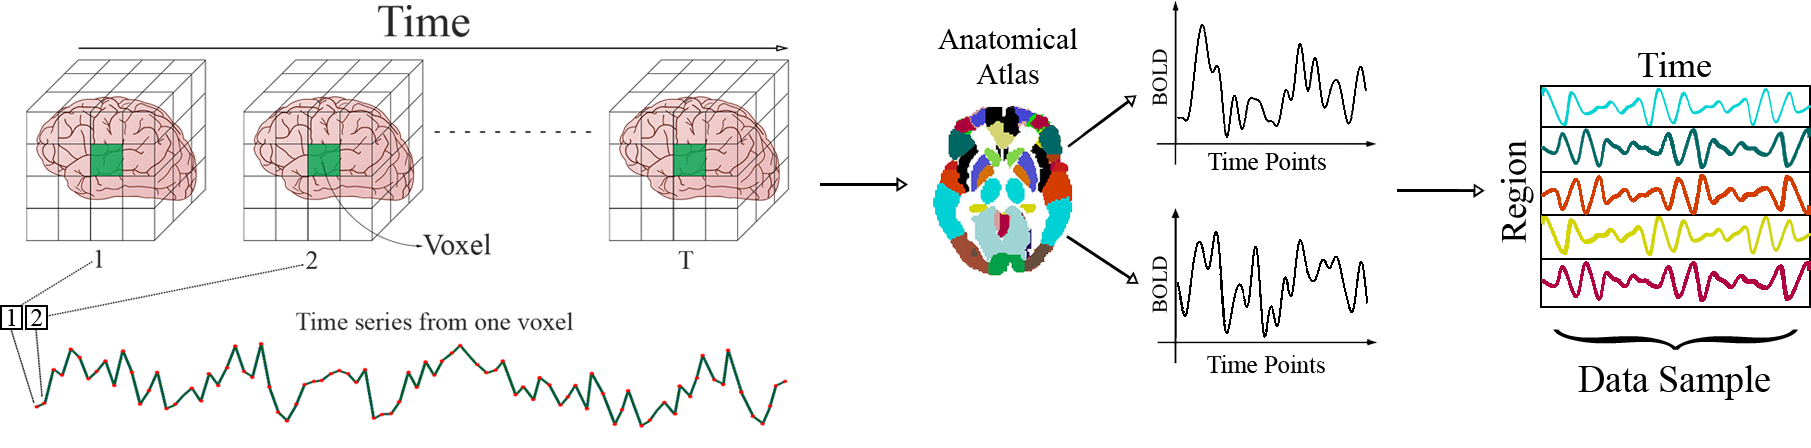
\includegraphics[width=6in]{Data}
		
		\caption{Simulation results for the network.}
		\label{g1.1}
	\end{figure*}
{\color{red}  * * * * * * * * * * * * * * * *}


in this paper we show that tensor representation is the natural form to present fMRI images. by this representation, we would be able to work with time and region features seperately in the same time. also with this representation we an easy and affordable multilinear dimension reduction that works with time and region features seperately this will be done by high order singular value decomposition of of the normal and eMCI subjects.
	
	also we show that by this representation and using the obtained HOSVD, dimension reduction step we can obtain tensor based discriminat features for classification. this discriminant method furthermore simplicity is very effective. here we show that by this framework the test data also could have effect in construction of discriminant function which is impossible in well known classification methods like SVM, logistic regression and etc. 
	
	by this approach the construction of FC feature that was time consuming is ignored and we represent an other method that at the same time with simple structure and low computation cost gives very high quality results with the other state of the art methods. 
	
	in fMRI data, one other feature is the fnctional connectivity of normal and abnormal subjects. as the third innovation of this paper we showed that based on hosvd of normal and eMCI patients and effective and high quality functional connectivity network can be extracted for both classes. we will show that some connectivities that are discovered via these FCs are well studied in recent clinical documents and thus . . . 
	
	%%ostad 3
	
	
	Distinguishing two rs-fMRI volumes in the machine learning viewpoint can be considered as a two class classification problem.
	%
	%in the first view, usualy and fMRI image in learning is considered as a time x region matrix $X_i \in T \times R$.
	Some methods use the vectorized version of samples ie, $x_i = vec(X_i)\in \mathbb{R}^T$ as  inputs of the learning process. However as we will discuss later, this vectorization may cause the loss of some important properties within the structure of data, and because of that the dominant approaches tend to find different set of features for each sample. These methods  construct a $region \times region$ matrix $\bar{X}_i \in \mathbb{R}^{R \times R}$ which is often called functional connectivity (FC) matrix and indicates the between correlation of ROIs. Since in most fMRI samples the number of timepoints is larger that the number of ROIs i.e.  $ T  > R$, substituting $X_i$ with $\bar{X}_i$ reduce the number of features and the effects of the \textit{curse of dimensionality}, also 
	it has been shown that using FC can enhance small between region connections hence turns FC into a powerful tool for rs-fMRI data analysis. For correlation computation, different methods have been explored, among which the pairwise Pearson’s correlation coefficient \cite{r10, r11}, sparse representation \cite{r10, r12, r13}  and Sparse Inverse Covariance Estimation (SICE) are of the popular ones \cite{r14, r15}. While the first two are easy to understand and can capture pairwise functional relationship based on a pair of ROIs, the latter can account for more complex interactions among multiple ROIs, but the estimation of partial correlation involves an inversion of a covariance matrix, which may be ill-posed due to the singularity of the covariance matrix. On the other hand, computing the correlation based on the entire time series of RS-fMRI data simply measures the FC between ROIs with a scalar value, which is fixed across time. This actually implicitly hypothesizes the stationary interaction patterns among ROIs. As a result, this method may overlook the complex and dynamic interaction patterns among ROIs, which are essentially time-varying \cite{r16}\textendash \cite{r19}.
	In order to overcome this issue, some methods have been proposed that consider the time as a non-stationery property. As for an example [] uses sliding-window technique in order to divide the time series into several smaller parts and then calculate the between correlation of these parts.[][] although these methods show promissing classification results, they are not computational favorable and since the aspect of region is not preserved in the final model, the relation between the high-order FC and the real world FC is somewhat ambigues. After calculating the FC, conventional classifiers like SVM or KNN is deployed in order to classify the vectorized FC for each sample \cite{r20}. 
	
	Although FC grants us certain useful structural properties such as being SPD and having relatively low dimensionality, using  it in the classification process has its own drawbacks such as calculating the proper FC and extracting key features from it. Considering these issues we have come up with a framework that eliminate the need for finding the FC in the classification process. Also the proposed framework works directly with the sample matrix and preserve its structural integrity by avoiding the vectorization using novel multilinear techniques.    
	(more about vectorization?)
	
	In this paper we claim that by considering $X_i \in \mathbb{R}^ {T \times R}$ as the sample, the dataset could be considered as an order three tensor. Using this representation we have shown that by extremely lower computational cost compared with other methods, and without the need to construct FC, a framework can be designed that only by one High Order Singular Value Decomposition (HOSVD) for each class could give us the desired results. This framework which we call it \textbf{TBNA} (High Order Feature Selection and Extraction) does three main tasks: 
	\begin{itemize}
		\item
		\textbf{Dimension Reduction:}
		The proposed frameworks allows us to select key features of each mode  (i.e. \textit{Time}, \textit{Region} and \textit{sample}) of the constructed tensor seperately and differently. This feature extraction would cause a massive reduction of the dimensions.
		
		\item
		\textbf{Classification:} 
		Based on the properties of the HOSVD, we have eliminated the vectorization at any step and hence assure that no information is lost in the vectorization process. Moreover we have formed a novel  classification enhancement technique that allows the test samples to cooperate in the training phase. This technique increases the tendency of the test sample to it's true class without forcing any apriory knowledge about it's label to the trainer. 
		
		\item
		\textbf{Functional Connectivity Network Construction:}
		Being able to see the class as a whole ables us to derive a Functional Connectivity network for each class. Such FCs allows us to investigate on shared properties within each class such as functional abnormalities of some ROIs or the connection between them.  
		
	\end{itemize}
	
	change
	
	
	%The novelty of this paper can be categorized in two cases:  The dimension reduction of fMRI samples, and the enhanced classifier. 
	
	To verify our approach, we conduct an extensive experimental study on rs-fMRI data from the
	benchmark dataset ADNI\footnote{http://adni.loni.usc.edu/} As will be seen, the results well demonstrate the effectiveness and advantages of our method. Specifically, the proposed TBNA system, not only grants us superior classification accuracy to that from other methods, it is also much faster. We have also confirmed our achieved FC matrix using empirical data on the eMCI functional connectivity patterns.
	
	
	%The rest of the paper is organized as follows: Section II contains the . In section III contains some basic concepts. We propose our novel Framework based on High order SVD and our classification enhancement method. And section IV presents some experimental results.   
	
	%%Dr.Rezghi
	
	
	
	%this new structure can be seen in figure **
	%which is mixed together in traditional methods 
	%
	%based on this representation of fMRI data, we would like to use the advantage of this multilinear representation to design multilinear analysis tool to deal with this data in the following we show that by using HOSVD:
	%
	%\begin{enumerate}
	%	\item 
	%	we can find dimension reduction which works with time and region features seperately
	%	\item 
	%	by this decomposition and without any extra computation cost, we design a new discriminant function that is able to classify the data based on HOSVD. 
	%	\item 
	%	in the end we show that by this decomposition, easily an FC for normal and eMCI can be obtained
	%\end{enumerate}
	%
	%
	%based on this representation of data, we would like to use the advantage of this multiview representation to design multilinear analysis tool to deal with this data. in the following we show that by using hosvd decomposition we should find dimension reduction which works with time and region features separately. 
	%
	%by this decomposition without extra computational cost, we design a new discriminant function that able to classify the data based on hosvd. 
	%
	%in the end we show that by this decomposition easily an FC fir normal and eMCI classes can be obtained. 
	%%Dr.Rezghi
	
	
	\section{Related Works}
	
	
	\subsection{Tensor Factorization and tensor learning} 
	is a higher-order extension of matrix
	factorization that elicit intrinsic multi-way structure and capture the underlying patterns in tensor data. There are
	many excellent works for tensor factorization The two most commonly used factorization techniques are CP and Tucker. Compared to Tucker, CP is more frequently used due to its properties of uniqueness and simplicity. A comprehensive survey on
	tensor factorization can be found in. However, the existing works are mainly based on multilinear factorization schemes, and are difficult to model nonlinear relationships and to discover complex patterns in data.
	Supervised tensor learning has been extensively studied
	in recent years. For example, proposed a supervised
	tensor learning framework, which extends the standard
	linear SVM learning framework to tensor patterns by constructing multilinear models. Under this learning framework,
	several linear tensor-based models
	are developed, whereas the problem of how to build nonlinear
	models directly on tensor data has not been well studied.
	In order to apply kernel modeling for tensor data, several
	works have been presented to convert
	the tensors into vectors (or matrices), which are then
	used to construct kernels. However, this kind of conversion
	will result in the following two problems: 1) break
	the natural multi-way structure and correlation in the original
	data; 2) lead to the curse of dimensionality and
	small sample size problems. The problem of how to
	build kernel modeling directly on tensor data has not been
	well studied. Most recent attempt in this direction is related
	to CP factorization proposed in, while it has the same
	drawback as CP factorization.
	
	\subsection{Brain network classification:}
	Classification techniques has been one of the most powerful tools in order to investigate in brain diseases. Here we briefly explain two state of the art methods which differs in their core hypothesis which is the stationary property of time in order to construct the FC.  
	
	\subsubsection{Compact SICE}
	In this method, first the SICE matrix is extracted from the data sample $S$ using the following optimization: 
	\begin{align}
	S^* = \operatorname{arg} \max\limits_{S\succ 0} \hspace{3mm} \log \left( \det(S) \right) - \operatorname{tr}(CS) - \lambda \norm{S}_1
	\end{align}
	where $C$ is the sample-based covariance matrix; $\det(·)$, $\operatorname{tr}(·)$,
	and $\norm{.}_1$ denote the determinant, trace, and the sum of the absolute values of the entries of a matrix. Since the dimensions of SICE matrix is $R^2$, with $R$ representing the number of ROIs, the obtained matrix is still relatively large. Principal Component Analysis(PCA) has proved itself to be one of the most powerful methods of dimension reduction and this method uses Kernel-PCA with a Gaussian kernel in order to extract the key features of SICE.
	Since SICE is an SPD matrix, specific distance functions such as Log-Euclidean distance or Root Stein divergence can be used as the distance function in the Gaussian kernel.
	After extracting key features, conventional methods like SVM or Knn could be deployed for classification.
	
	\subsubsection{High Order Networks(HON)}
	This method uses so called High Order Networks as features for classification purposes. it uses the sliding window technique in order to split the time-series into smaller pieces and then find the relation between them. Let $x_{i}^{(l)}(k) \in \mathbb{R}^N$ denote the $k$-th segment of subseries extracted from $x_{i}^{(l)}$, which comprises $N$ image volumes. by taking each $x_{i}^{(l)}(k)$ as a node A network can be constructed with edges defined using:
	\[
	C_{ij}^{(l)}(k) = \operatorname{corr}\left(x_{i}^{(l)}(k),x_{j}^{(l)}(k)
	\right)
	\]
	which represents the pairwise Pearson’s correlation coefficients
	between the $i$-th and the $j$-th ROIs of the $l$-th subject using the $k$-th segment of subseries. 
	%\[
	%G_l^{(l)}(k) = \left( 
	%\{ x_i^{(l)}(k) \} , \{ C_{ij}^{(l)}(k) \}
	%\right)
	%\]
	by taking  
	\[
	y_{ij}^{(l)} = \left[ 
	C_{ij}^{(l)}(1), C_{ij}^{(l)}(2), \cdots , C_{ij}^{(K)}(1) 
	\right] \in \mathbb{R}^K
	\]
	as new nodes, an other network can be calculated as follow: 
	\[
	H_{ij,pq}^{(l)} = \operatorname{corr} \left(
	y_{ij}^{(l)},y_{pq}^{(l)}
	\right)
	\]
	for each pair of correlation time series $y_{ij}$ and $y_{pq}$ thus, $H_{ij,pq}^{(l)}$ indicates how the correlation between the $i$-th and the $j$-th ROIs influence the correlation between the $p$-th and the $q$-th ROIs.
	The total number of the high-order correlation coefficients
	$\{ H_{ij,pq}^{(l)} \}$ is proportional to $R^4$ which will lead to a large-scale high-order FC
	network, containing at least thousands of vertices and millions
	of edges. In order to overcome this issue, the correlation time series within each subject is grouped into different clusters. Then, the correlation calculation
	between the original correlation time series can be
	converted into that between the respective mean correlation
	time series in clusters. After reducing the network size, the
	weighted-graph local clustering coefficients was used to select the key features for each network and then SVM is used in order to classify the obtained features.  
	
	\section{Preliminaries} \label{Chap_3}
	In this section, we briefly introduce some preliminary knowledge from tensor algebra. For a deeper introduction
	to the concepts and terminology, we refer to [17]. Before proceeding, we introduce some basic notations that will be used throughout this paper.
	Tensors (\textit{i.e.}, multidimensional arrays) are denoted by
	calligraphic letters ($\mathcal{A}, \mathcal{B}, \mathcal{C}, \cdots$), matrices by boldface
	capital letters $(\boldsymbol{A, B, C, \cdots})$, vectors by boldface lowercase letters $(\boldsymbol{a, b, c, \cdots})$, and scalars by lowercase
	letters $(a, b, c, \cdots)$. The columns of a matrix are denoted by boldface lower letters with a subscript, \textit{e.g.}, $\boldsymbol{a}_{i}$
	is the $i$th column of matrix $\boldsymbol{A}$. The elements of a
	matrix or a tensor are denoted by lowercase letters with
	subscripts, \textit{i.e.}, the $(i_1, \cdots, i_n)$ element of an $n$-th order
	tensor $\mathcal{A}$ is denoted by $a_{i_1, \cdots, i_n}$. In formulas we will sometimes
	use MATLAB-style notations. For instance, we define
	the mode-1 fibers of a 3-tensor $\mathcal{A}$ to be the column vectors $\mathcal{A}(:, j, k)$.
	
	\begin{figure}[!t]
		\centering
		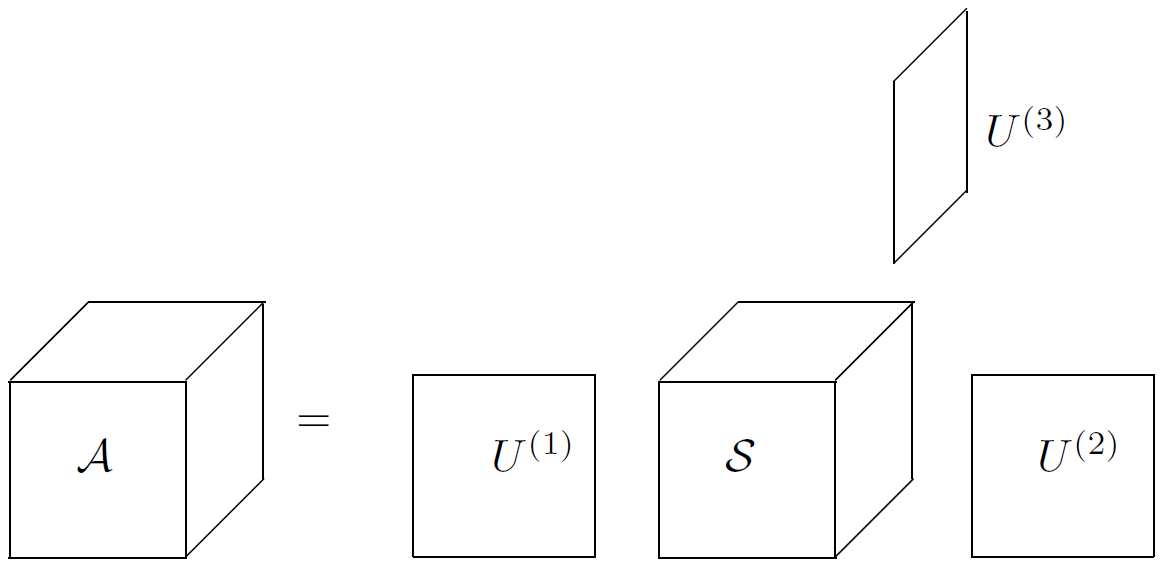
\includegraphics[width=3in]{HOSVD}
		
		\caption{Simulation results for the network.}
		\label{g2.1}
	\end{figure}
	
	\subsection{Basic Tensor Operations}
	Let $\mathbb{R}^{I_1\times \cdots \times  I_M}$ be endowed with the usual Euclidean geometry and $\mathcal{A}  \in \mathbb{R}^{I_1\times \cdots \times  I_M}$. where $I_k$'s are positive integers; the vector space $\mathbb{R}^{I_1\times \cdots \times  I_M}$
	has dimension ${I_1\times \cdots \times  I_M}$, and $\mathcal{A}$ is a tensor in this space. If $M = 2$, $\mathcal{A}$ would be a matrix in $\mathbb{R}^2$.
	
	A fiber is a subtensor, where all indices but one are fixed. For
	example mode-2 fibers of $\mathcal{T} \in \mathbb{R}^{I_1 \times I_2 \times I_3 }$, have following form
	\[
	\mathcal{T}(i_1,:,i_3)\in \mathbb{R}^{I_2}
	\]
	
	Similarly, we define \textit{slices} of a tensor to be the sub-tensors obtained by fixing the index in one mode, \textit{e.g.} 
	\[
	\mathcal{T}(:,i_2,:)\in \mathbb{R}^{I_1 \times I_3}
	\]
	is an slice of $\mathcal{T}$ in mode-2. 
	
	The mode-$n$ product of an order-M tensor $\mathcal{A}  \in \mathbb{R}^{I_1 \times \cdots \times I_M}$ by a matrix $X \in \mathbb{R}^{K \times I_n}$ is defined as 
	
	\begin{align}\label{f2.1}
	\mathcal{B} = (X)_n \boldsymbol{\cdot}	A \in \mathbb{R}^{I_1 \times \cdots \times I_{n-1} \times K \times I_{n + 1} \times \cdots \times I_M}
	\end{align}
	where,
	\[
	b_{i_1, \cdots, i_n} = \sum_{l = 1}^{I_n} x_{i_n, l} a_{i_1,\cdots, i_{n-1}, l, I_{n+1}, \cdots I_M }.
	\]
	This means that all mode-$n$ fibers of $\mathcal{A}$ are multiplied by the
	matrix $X$. The notation \eqref{f2.1} was suggested by Lim [23]. An alternative notation was earlier given in [24]. $ (X)_n \boldsymbol{\cdot}	A$ is the same as $\mathcal{A} \times_n X$ in that system. 
	
	The Frobenius norm of the order-$M$ tensor $\mathcal{A}$ can also be defined as 
	\[
	\|  \mathcal{A} \| = \left( \sum_{i_1, \cdots, i_m} a^2_{i_1, \cdots i_m} \right)^{1/2} .
	\]
	
	
	\subsection{Matricization}
	Sometimes it is useful to rearrange the tensor into a matrix. A tensor can be \textit{matricized}\footnote{Alternative terms are \textit{unfolding} [9] or \textit{flattening} [13].} in many different ways[26], [27]. In special case rearranging the mode-$n$  fibers of a tensor $\mathcal{A}$ is an operation where the mode-$n$ fibers of $\mathcal{A}$ are aligned as the columns of a matrix, denoted $K^{(n)}$[26][27]. The mode-$n$ matricization $A^{ ( n; 1,\cdots n-1,n+1,\cdots ,M ) }$ is a map between the element $a_{i_1,\cdots i_n}$ of $\mathcal{A}$ to $(i_n, j)$ of the matrix $A^{(n)}$ where 
	
	\begin{align*}
	j = 1+\sum_{k=1, k \neq n}^{M}(i_k - 1)J_k, \quad J_k = \prod_{m =1, m\neq n}^{k-1} I_m
	\end{align*}
	
	\subsection{Higher order singular value decomposition}
	Higher order singular value decomposition (HOSVD) is
	one common extension of singular value decomposition to
	the tensors [24]. Using HOSVD, every order-$M$ tensor $\mathcal{A} \in \mathbb{R}^{I_1 \times \cdots I_M}$ can be decomposed as 
	\begin{align}\label{f2.2}
	\mathcal{A} = \left( U_{(1)}, \cdots, U_{(M)} \right) \boldsymbol{\cdot} \mathcal{S},
	\end{align}
	where orthogonal matrices $U^{(i)}$ are singular matrices of tensor $\mathcal{A}$. Here, $U^{(i)}$ is the left singular matrix of $\mathcal{A}^{(i)}$. The core
	tensor $\mathcal{S}$ is a real tensor of the same dimensions as $\mathcal{A}$ and 
	\begin{align}\label{f2.3}
	\mathcal{S} = \left( U_{(1)}^{T}, \cdots, U_{(M)}^{T} \right) \boldsymbol{\cdot} \mathcal{A}.
	\end{align}
	
	
	
	Although this core tensor is not diagonal as in the case of
	SVD of matrices, but satisfies the following conditions:
	\begin{itemize}
		\item Any two different slices along the same mode are orthogonal.
		This property of core tensor S is named as all orthogonality.
		\item The values $s_j^k = \| \mathcal{S}(:, \cdots, :, j, :, \cdots, :) \| $, where $j$ is in
		the $k$th mode of $\mathcal{S}$, are named mode-$k$ singular values of
		$\mathcal{A}$. It can be shown that for every $k$
		
		\begin{align}\label{f2.4}
		s_1^k \geq s_2^k \geq \cdots \geq s_n^k \geq 0, \quad k = 0, \cdots, M.
		\end{align}
		
		are equal to the singular values of the matrix $A^{(k)}$. This
		means that the norms of the slices along every mode are
		ordered. 
		
	\end{itemize}
	
	The ordering property \eqref{f2.2} demonstrates that, in the same
	way as matrices, singular values measure the 'energy' of the
	tensor. So, it is easy to see that the energy of core tensor $\mathcal{S}$
	focused on the elements of $\mathcal{S}$ with small indices, especially in $\mathcal{S}(1,1, \cdots, 1)$. HOSVD for a 3-tensor is illustrated in figure \eqref{g2.1}.
	
	
	
	The computation of the HOSVD of a tensor $\mathcal{A} \in \mathbb{R}^{I_1 \times \cdots \times I_M}$ can be done by separately computing the orthogonal matrices $U_{(1)}, U_{(2)},\cdots,  U_{(M)}$, as the left singular matrices of $A^{(m)}, m = 1, 2, \cdots M$. \textit{i.e.}:
	
	\begin{enumerate} 
		\item Compute the SVDs:
		\begin{align*}
		A^{(i)} &= U^{(i)}S^{(i)}(V^{(i)})^T,
		\end{align*}
		without forming the $V ^{(i)}$’s explicitly
		\item  Compute the core tensor: $\mathcal{S} =\left( U_{(1)}^{T}, \cdots, U_{(M)}^{T} \right) \boldsymbol{\cdot} \mathcal{A}$
	\end{enumerate}
	
	
	
	
	\section{Proposed fMRI analysis Framework}
	% needed in second column of first page if using \IEEEpubid
	%\IEEEpubidadjcol
	By using the properties of HOSVD, the proposed framework allows us to reduce the dimensionality of data, create a discriminant function and enhance it and also calculate an FC network. These four features are discussed in full detail in the following sections:
	
	
	%%Begin Dr.Rezghi Suggestions
	\subsection{Dimension Reduction and Feature Extraction}
	Let $x\in \mathbb{R}^n$ be a sample data, in this case, 
	$y = U^T_k x \in \mathbb{R}^k$ is a linear feature extraction and 
	$\bar{x}  = U_k U_k^T x$ denotes an approximation of $x$ in space spanned by base columns $\{ u_1,\cdots, u_k \}$. In fact $y$ is in a \textit{latent} space spanned by $\{ u_1,\cdots, u_k \}$, and 
	$\bar{x}$ is the filtered version of $x$ that in it only the effects of basis vectors $\{ u_1,\cdots, u_k \}$ are preserved. So by choosing appropriate values for $\{ u_1,\cdots, u_k \}$ we could remove the unnecessary parts of $x$ in the original space or in the feature space. These unnecessary parts can be accounted for noise or outliers in the data.
	
	When  samples are not vectors, two approaches can be followed, the first one is to simply vactorize the data and use linear feature extractors as described above. Although this approach is easy to deploy, it has several drawbacks, one main drawback would be the Curse of dimensionality that appears when the proportion of the number of features to the number of samples is relatively high (which results in over-fitting). 
	Also in this view different kind of features(like \emph{Time} and \emph{region} in our case) would be mixed together which may discard some important information within these features. The second approach is to deploy multilinear methods. 
	
	Due to the multilinear nature of our data, it seems natural to take advantage of multilinear
	techniques in order to reach  better performances. As we described before, each sample is considered to be 
	$X \in \mathbb{R}^{T \times R}$ where $x_{ij}$ is the $i$th observation of the $j$th node and thus the $i$th class can be considered as 
	$\mathcal{X}^{(i)}\in \mathbb{R}^{T \times R \times S_i}$ where 
	$\mathcal{X}(:,:,s)$ is the $ s $'th sample in the $i$th class. figure * shows this structure.
	Observing the dataset as a multilinear entity would allow us to treat each mode differently. Since each mode represents a different feature(e.g. \textit{time} or \textit{region}) appropriate dimension reduction methods can be deployed separately on each mode. 
	
	As an example of a multilinear feature extraction approach let: $\mathcal{X} \in \mathbb{R}^{I_1\times \cdots \times I_N}$ then
	\begin{align}\label{dimention_reduction}
	\mathbb{R}^{I_1 \times \cdots I_{i-1}\times k_i \times I_{i+1} \times \cdots \times I_N} \ni
	\mathcal{Y}  = (U_{k_i}^T)\boldsymbol{\cdot} \mathcal{X} 
	\end{align}
	is the dimension reduced version of $\mathcal{X}$ in the $i$th mode. We have also 
	\[
	\mathbb{R}^{I_1 \times \cdots \times I_N}
	\ni
	\bar{\mathcal{X}} = \left( U^{}_{k_i} (U^{}_{k_i})^T \right) \boldsymbol{\cdot} \mathcal{X} 
	\]
	that is the filtered version of $\mathcal{X}$ in the $i$th mode according to the basis matrices $\{ U_{k_1},\cdots, U_{k_i} \}$.  So
	based on the properties of each feature, both $Y$ and $\bar{X}$ can be used together in order to extract the features. 
	
	
	% Here $Y$ and $\bar{X}$ are named \textit{feature reduced} and \textit{filtred version} of $\mathcal{X}$ in the $i$th mode  according to the basis $\{ U^i_1,\cdots, U^i_{k_i} \}$.
	
	
	A key aspect in dimension reduction and feature extraction is finding the appropriate projection matrices $\{ U_1,\cdots, U_{k_i} \}$. When data samples are vectors, methods like 
	Non-negative Matrix Factorization(NMF), Principal Component Analysis(PCA) and Singular Value Decomposition(SVD) are traditionally used to obtain such basis vectors. As the number of dimensions grows and therefore the dataset becomes a tensor, multilinear methods (such as MPCA or HOSVD) should be deployed in order to extract the appropriate basis matrices.  As we mentioned before, HOSVD is a tensor decomposition technique that provides us with basis matrices for each mode of a tensor. 
	If we denote the $i$th class with 
	$\mathcal{X}^{(i)} \in \mathbb{R}^{T \times R \times S_i}$ in which $T$, $R$ and $S_i$ denotes the size of the \textit{Time}, \textit{Region} and \textit{Sample} modes respectively, then it's HOSVD would be:
	\[
	\mathcal{X}^{(i)} = 
	\left(  
	U_{1}^{(i)},U_{2}^{(i)},U_{3}^{(i)}
	\right)\boldsymbol{\cdot} \mathcal{S}^{(i)}
	\]   
	where for $k= 1,2,3$, $U_{k}$ is the mode-$ k $ singular matrix of $\mathcal{X}^{(i)}$, and $S^{(i)}$ is the core tensor. As it was mentioned in \eqref{Chap_3} $U_{1}$ is a base of all mode-$ 1 $ fibers $\mathcal{X}^{(i)}(:,i,j)$ which indicates the behavior of $i$th region of the $j$th sample in all times. 
	Also due to the properties of HOSVD inherited from svd, the first columns of $U_{i}$ has more ability in construction of main parts of $i$th fiber and on the other hand, the last columns of  $U_{i}$ in each mode, are corresponding to noise parts of these fibers and hence projecting the data in mode-$ i $ into space of $U_{k} = \left[ u_{1}, \cdots, u_{k_i} \right]$
	is a suitable dimension reduction. For example,
	\[
	\mathbb{R}^{k \times R\times S} \ni \mathcal{X}_f = \left(U_{k_1} \right)_1^{\trans} \boldsymbol{\cdot} \mathcal{X} 
	\]
	is a dimension reduction in the first mode of $\mathcal{X}$. Note that $\mathcal{X}_f$ is in the feature space induced by  $\left( U_{k_1} \right)^{\trans}$.
	%As an example for the filtering in the first mode based on the singular matrix $U^{(1)}$, $\mathcal{X}$ can be written as 
	%\begin{align}
	%\mathcal{X} = \left( U_{k}^{(1)} \right)\boldsymbol{\cdot} &\left(  
	%(U^2, U^3)_{2,3}\boldsymbol{\cdot} \mathcal{S} (  \left[ K \right] , :,: )
	%\right)	+\\
	%&\left( U_{\bar{k}}^{(1)} \right)\boldsymbol{\cdot}
	%\left(  
	%(U^2, U^3)_{2,3}\boldsymbol{\cdot} \mathcal{S} (  \left[ \bar{K} \right] , :,: )
	%\right). \notag
	%\end{align} 
	% the second part of the above summation can be eliminated due to the fact that the last columns of $U^{(i)}$ are less stable and also in the reconstruction process they are multiplied by  $\mathcal{S} (  \left[ \bar{K} \right] , :,: )$ which contains small values. Thus
	% \[
	% \bar{\mathcal{X}} = \left( U_{k}^1 \right)\boldsymbol{\cdot} \left(  
	% (U^2, U^3)_{2,3}\boldsymbol{\cdot} \mathcal{S} (  \left[ K \right] , :,: )
	% \right)
	% \]
	%would be the filtred version of $\mathcal{X}$ in the first mode.       
	
	let $X^{(i)} \in \mathbb{R}^{T \times R \times S_i}$ denotes the $i$th class. using HOSVD on each class, using the mensioned DR method, the $i$th class becomes: 
	\[
	\bar{\mathcal{X}}^{(i)} = \left(
	U_{1}^{(i)}(1:k_1^i, :)^{\trans}, U_{2}^{(i)}(1:k_2^i, :)
	\right) \boldsymbol{\cdot} \mathcal{X}^{(i)}
	\]
	
	\subsection{Discriminant Function}
	%% DR. Rezghi version
	In  previous section we proposed a novel framework for feature extraction and dimension reduction of fMRI data. We have also introduced a classification technique to distinguish eMCI and Normal subjects. In our case, classifiers like SVM, knn and other convenient classifiers or their multilinear versions such as STM could be applied.
	Since even in atlas-based approach the number of features are relatively high, the computation cost of the mentioned classifiers are also high and would probably cause the over-fitting issue. 
	
	In this section, using the computed components of HOSVD from the last section, and without extra computational costs, we have designed a discrimination process. 
	Let $\mathcal{X} = \left( U_{(1)}^{i},U_{(2)}^{i},U_{(3)}^{i} \right)$ denotes the HOSVD of the $i$th class, its correspondent dimension reduced tensor would be 
	\begin{align}
	\mathbb{R}^{k_1^i \times k_2^i \times S} \ni  \bar{{\mathcal{X}}} = \left( 
	{U_{k_1^i}^{(i)}}^{\trans}, {U_{k^i_2}^{(i)}}^{\trans} 
	\right)_{1,2}\boldsymbol{\cdot} \mathcal{X} \label{DR_Version}
	\end{align}
	where the $U_{k_1^i}^{(i)}$ and $U_{k_2^i}^{(i)}$ are the first $k_1^i$ and $k_2^i$ vectors of the singular matrix $U_1^{(i)}$ and $U_2^{(i)}$ respectively. by \eqref{DR_Version} the above equation can be written as 
	\begin{align}
	\bar{\mathcal{X}}= & \notag
	\left(
	\begin{bmatrix}
	I_{k_1^i} &  0
	\end{bmatrix},
	\begin{bmatrix}
	I_{k_2^i} &  0
	\end{bmatrix},
	U_3^{(i)}
	\right)\boldsymbol{\cdot} \mathcal{S} \notag
	\\&=\left( 
	U_{3}^{{(i)}}
	\right)_{3} \boldsymbol{\cdot} \mathcal{S}(1:k_1^i, 1:k_2^i, :) \notag &
	\end{align}
	
	%%ostad
	in the next step we develope our multilinear classification method based on HOSVD. from 7 it is easy to show 8. 
	
	\begin{align*}
	\bar{{\mathcal{X}}}^{(i)}(:,:,k) &= \sum_{k' = 1}^{S_i} U_{3}^{(1)}(k,k') \boldsymbol{\cdot} \mathcal{S}(1:k_1^i, 1:k_2^i, k')\\
	&=\left(  
	U_3^{(i)}(k,:)
	\right)_{3} \boldsymbol{\cdot} \mathcal{S}(1:k_1^i, 1:k_2^i, :)
	\end{align*}
	by this equation and by increasing $k'$ from HOSVD we know that $\mathcal{S}(1:k_1^i, 1:k_2^i, k')$ becomes smaller also the $U_{3}^{(1)}(k,k')$ for large $k'$ show ossilated behaviour.
	%%ostad
	
	
	it is clear that the $k$th sample from the $i$th class in the new feature space can be written as $\bar{\mathcal{X}}^{(i)}(:,:,k)$, thus we have:
	\begin{align}
	\bar{\mathcal{X}}^{(i)}(:,:,k) &= \sum_{k'}^{N_i} U_3^{(i)}(k,k')\bar{\mathcal{S}}^{(i)}(:,:,k') \notag
	\\&= \left( U_{3}^{(i)}(k,:)\right)_3 \boldsymbol{\cdot} \bar{\mathcal{S}}^{(i)}
	\end{align}
	in which 
	\[
	\bar{\mathcal{S}}^{(i)} = \mathcal{S}(1:k_1^i, 1:k_2^i, :)
	\]
	this means that all elements in the $i$th class in the new domain can be reconstructed by the slices of $\bar{\mathcal{S}}^{(i)}$. Also by the properties of the core tensor we know that the first slices of $\bar{\mathcal{S}}^{(i)}$ Has higher value and since they are multiplied by the first columns of singular matrices, they have higher effects in the reconstruction process so by truncating the $\bar{\mathcal{S}}^{(i)}$ tensor we would have: 
	\begin{align}
	\bar{\mathcal{X}}^{(i)}(:,:,k) &\approx \sum_{k'}^{l} U_3^{(i)}(k,k')\bar{\mathcal{S}}^{(i)}(:,:,k') \notag
	\\&
	= \left( U_{3}^{(i)}(k,1:l)\right)_3 \boldsymbol{\cdot} \bar{\mathcal{S}}^{(i)}_l \label{Basis} 
	\end{align} 
	where
	\[
	\bar{\mathcal{S}}^{(i)}_l = \mathcal{S}(1:k_1^i, 1:k_2^i, 1:l)
	\]
	
	
	These relations helps us to design a novel discreminant function. Since every sample in the $i$th class could be reconstructed by $\bar{\mathcal{S}}^{(i)}_l$ to assign a test data $Z \in \mathbb{R}^{T \times R}$ to a class we can do the following process: First we project the $Z$ matrix to the span of singular matrices of the two available classes:
	\begin{align}
	\bar{Z}^{(i)} &= \left( 
	{U_{k_1^i}^{(i)}}^{\trans},  {U_{k_2}^{(i)}}^{\trans} 
	\right)_{1,2} \boldsymbol{\cdot} Z \notag \\
	&= {U_{k_1^i}^{(i)}}^{\trans} Z \hspace{2mm} U_{k_2^i}^{(i)}\label{DR_test}
	\end{align} 
	in which $\bar{Z}^{(i)}$ denotes the test data $Z$ after pruning with respect to the $i$th class. 
	The coordinates of $\bar{Z}^{(i)}$ in the extracted basis of the $i$th class can be obtained via:
	\begin{align*}
	x^i =\operatorname{arg} \min_\mathrm{x} \norm{\bar{Z}^{(i)} - \sum_{j} x_j X_{j}^i  } 
	\end{align*}
	in which $X_{j}^i$ is %$\bar{\mathcal{X}}^{(i)}(:,:,j)$ 
	the $j$th frontal slice of $\bar{\mathcal{X}}^{(i)}$. The above minimization is equivalent to: 
	\begin{align*}
	\min_x \norm{B^i x -z^i }
	\end{align*} 
	in which 
	$b^i_j = \operatorname{vec}(A^i_{j})$
	and
	$z^i = \operatorname{vec}(\bar{Z}^{(i)})$. 
	%And thus
	%\begin{align*}
	%x^i = \left( (B^i)^{\trans} B^i + \lambda I  %\right)^{\dagger} (B^i)^{\trans} z
	%\end{align*} 
	Now we can argue that $\bar{Z}^{(i)}$ belongs to the class $c = \operatorname{arg} \min_\mathrm{i} \{ r_i\}_{i = 1}^{I}$,
	in which 
	\begin{align}
	r_i = \norm{z^i - B^i x^i} \label{Residual}
	\end{align}
	
	
	\subsection{Enhancement of the Discriminant Function}
	The designed framework allows us to involve the test subject in the training process without inducing any apriory knowledge about its label to the discriminant function. As it was discussed in the previous section, each sample in a class can ideally be reconstructed via the frontal slices of $\bar{\mathcal{S}}^{(i)}_l$ which itself is obtained via HOSVD. Based on this decomposition for the $i$th class $\mathcal{X}^{(i)}$ we can see that: 
	\begin{align}
	\mathcal{X}^{(i)} = \left( U_{k_3} \right)\boldsymbol{\cdot} &\left(  
	(U_{(1)}, U_{(2)})_{1,2}\boldsymbol{\cdot} \bar{\mathcal{S}}^{(i)}_l
	\right)	+ \notag \\
	&\left( U_{\bar{k}_3} \right)\boldsymbol{\cdot}
	\left(  
	(U_{1}, U_{(2)})_{1,2}\boldsymbol{\cdot} \bar{\mathcal{S}}^{(i)}_{\bar{l}} 
	\right). \label{dec}
	\end{align}
	in which
	\begin{align}
	\bar{\mathcal{S}}^{(i)}_l &= \mathcal{S}(1:k_1^i, 1:k_2^i, 1:l)\notag
	\\
	\bar{\mathcal{S}}^{(i)}_{\bar{l}} &= \mathcal{S}(k_1^i:end, k_2^i:end, l:end)\notag
	\end{align}
	we have chosen the frontal slices of $\bar{\mathcal{S}}^{(i)}_l$ to be the basis matrices for the $i $th class since it contains the shared information between samples, and discarded $\bar{\mathcal{S}}^{(i)}_{\bar{l}}$ since it probably contains noise and other non-common information within individual samples. 
	
	In order to enhance the obtained basis for each class, the test data $Z$ is appended to each class before the basis extraction process. Doing such has two possible effects: If $Z$ share common patterns with other samples, it will mostly affect the first part of \eqref{dec}, i.e. $\bar{\mathcal{S}}^{(i)}_l$. The second possibility is that $Z$ is not similar to other subjects and hence it will mostly effect the second part of \eqref{dec}, i.e. $\bar{\mathcal{S}}^{(i)}_{\bar{l}}$. This effect is due to the fact that by the properties of HOSVD, the common patterns manifest themselves in the first singular matrices and their corresponding basis matrices. Figure \eqref{g3.1} shows a better demonstration of this effect. As it can be seen in this figure, when the test data is similar to the rest of the class the first singular values get heavily affected, on the other hand when the new data does not show similarity to the rest subjects in the class it affects the last singular values which will be discarded along with their corresponding basis matrices.
	
	In order to better demonstrate the classification process
	it is summarized in algorithm \eqref{alg_1}.
	
	\begin{figure}[!t]
		\centering
		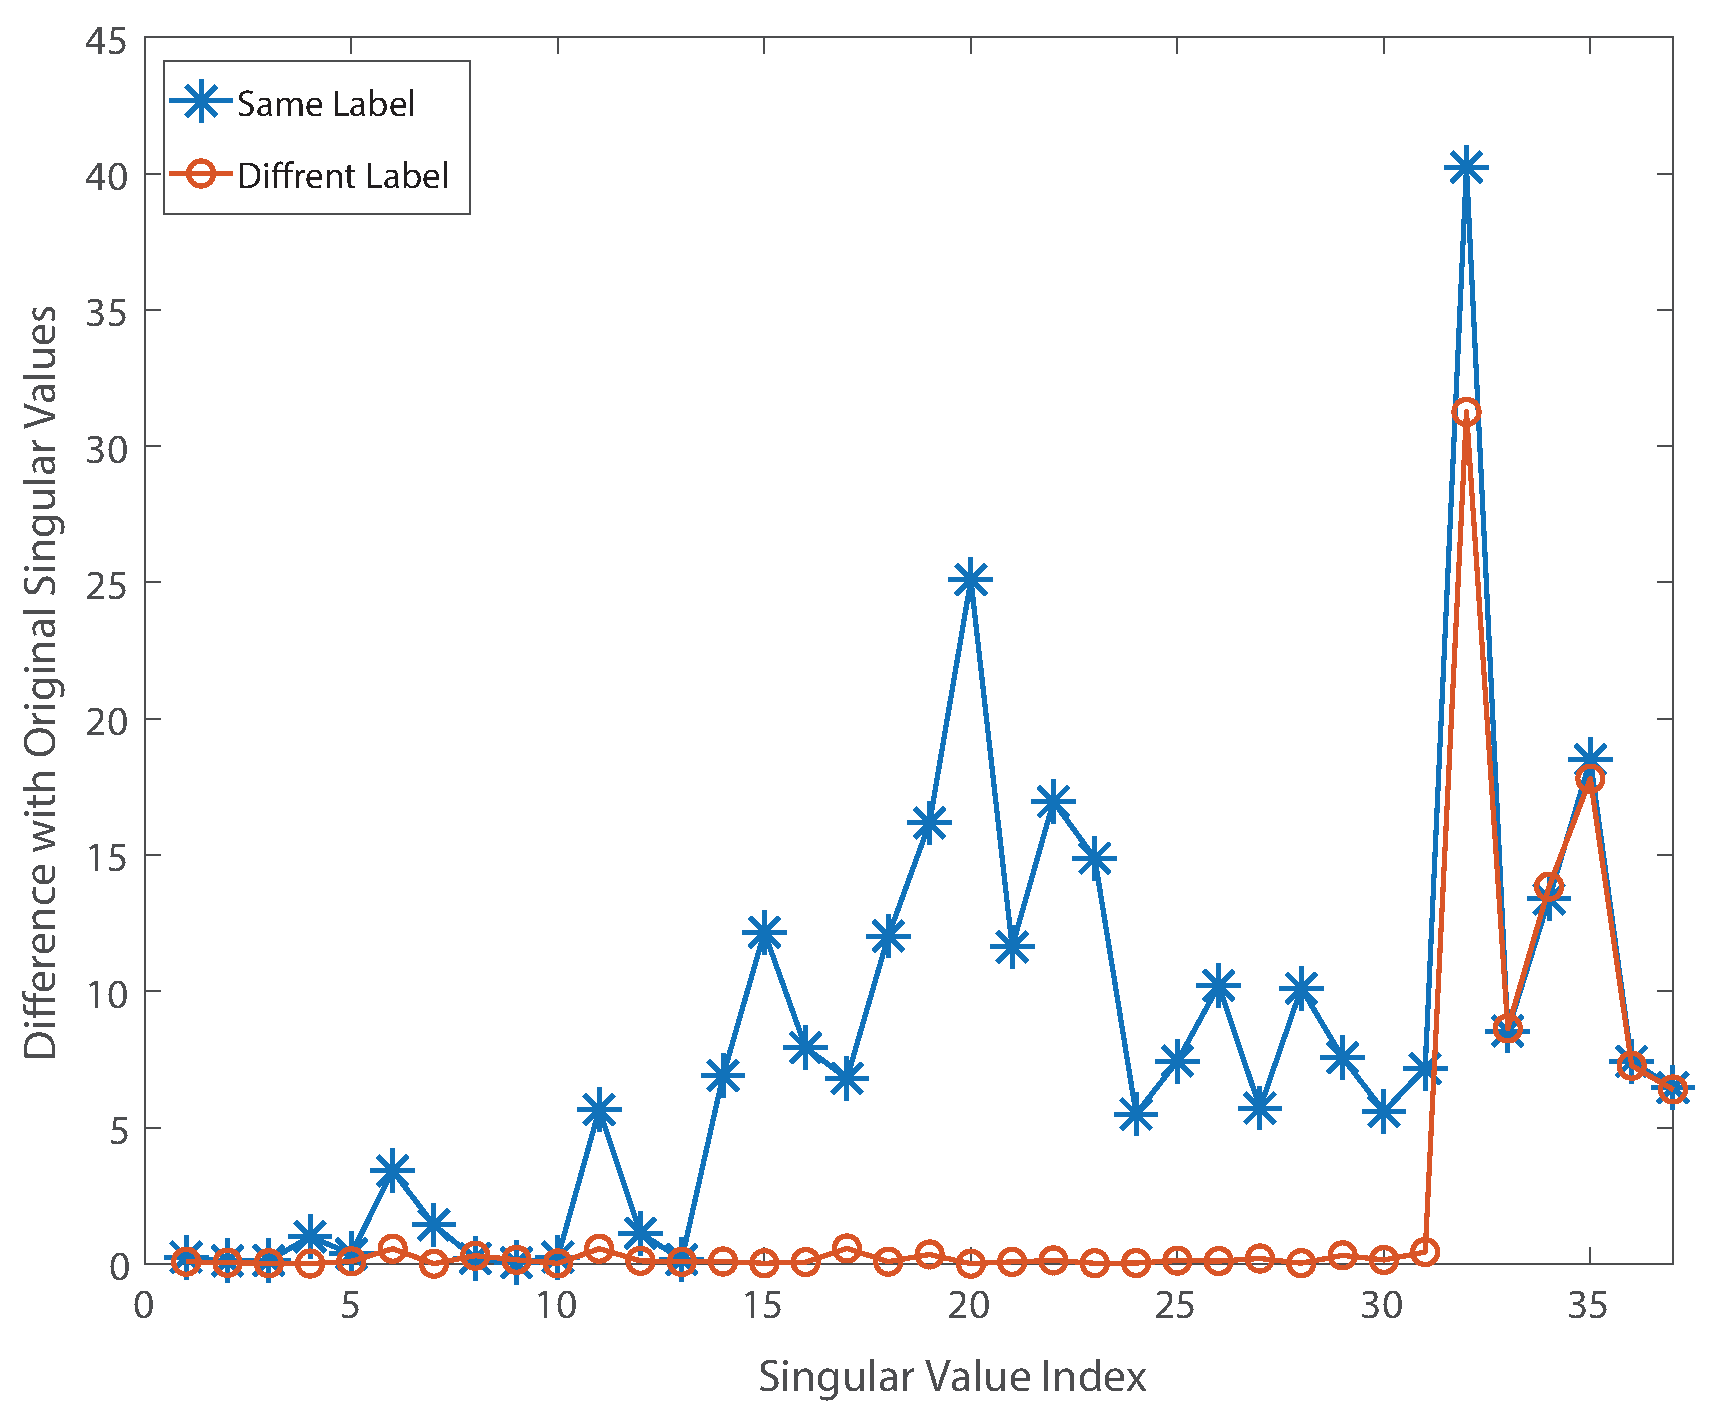
\includegraphics[width=3.5in]{SVDiff}
		
		\caption{The blue line with the star indicator, shows the difference between the mode-$3$ singular values of the original data and the data appended with a \emph{same} label subject. The orange line indicated with circles, shows the difference between the mode-$3$ singular values of the original data and the data appended with a \emph{different} label subject.}
		\label{g3.1}
	\end{figure}
	
	
	\begin{algorithm} 
		\label{alg_1}
		\SetAlgoLined
		\KwData{$\mathcal{X}^{(1)},\cdots,\mathcal{X}^{(I)}\in \mathbb{R}^{T \times R \times S}$, $Z\in \mathbb{R}^{T\times R}$}
		\KwResult{Label of $Z$}
		\For{$i\leftarrow 1$ \KwTo $I$}{
			Append the test data $Z$ to tthe $i$th class
			\\Calculatethe \emph{basis} $\bar{\mathcal{S}}^{(i)}_l$ of the $i$th class
			\\Calculate $\bar{Z}^{(i)}$ based on \eqref{DR_test}
			\\Calculate and store $r_i$ based on \eqref{Residual}
		}
		\Return{ $c = \operatorname{arg} \min_\mathrm{i} \{ r_i\}_{i = 1}^{I}$ }
		\\
		\caption{Classification by TBNA}
		\vspace{3mm}
	\end{algorithm} 
	
	
	
	\subsection{Functional Connectivity} \label{FC_Construction}
	Functional connectivity simply means the relation between different ROIs. Although several approaches have been proposed in order to find the functional connectivity, the majority of them focus on the individual samples rather that the whole class. This may overlook tiny but common connectivities shared within a class like the class of people in their early Alzheimer's disease.  
	
	The proposed framework allows us to obtain an FC network for each class. Although we do not use the FCs in the classification process, FC networks would allow further investigations on the brain activities. Let $\mathcal{X} \in \mathbb{R}^{T \times R \times S}$, finding the FC for this class means finding the relation between mode-2 slices of $\mathcal{X}$. Viewing each region as a slice would allow us to consider it's behavior in all time points and across all samples, which itself allows us to shed more light on common properties and ignore individual differences that is highly possible due to the presence of noise and outliers. 
	
	In order to calculate the FC, we first reduced the dimensions of our data similar to what we did in the previous part: 
	\begin{align}
	\mathbb{R}^{k_1^i \times R \times k_3^i} \ni  \bar{{\mathcal{X}}} = \left( 
	{U_{k_1^i}^{(i)}}^{\trans}, {U_{k^i_3}^{(i)}}^{\trans} 
	\right)_{1,3}\boldsymbol{\cdot} \mathcal{X} \label{DR_Version_FC}
	\end{align}
	it can be seen that each region slice can be written as:
	\begin{align}
	\bar{\mathcal{X}}^{(i)}(:,k,:) &= \sum_{k'}^{N_i} U_2^{(i)}(k,k')\bar{\mathcal{C}}^{(i)}(:,k',:) \notag
	\\&= \left( U_{2}^{(i)}(k,:)\right)_2 \boldsymbol{\cdot} \bar{\mathcal{C}}^{(i)}
	\end{align}
	in which 
	\[
	\bar{\mathcal{C}}^{(i)} = \mathcal{C}(1:k_1^i,:,1:k_3^i).
	\]
	Thus the $k$th mode-2 slice of $\mathcal{X}$, i.e. the $k$th region, can be written as the linear combination of 
	
	in order to extract low dimensional features for each region, they were reconstructed via the obtained basis matrices and their coefficients were stored as the new representative for each region. In order to do such, each region should be transfered to the space of basis matrices, let the $i$th region be $B = \mathcal{X}(:,i,:)$ then the transfered version would be
	\[
	\bar{B}^{(i)} = \left( 
	{U_{k_1^i}^{(i)}}^{\trans},  {U_{k_3}^{(i)}}^{\trans} 
	\right)_{1,3} \boldsymbol{\cdot} B 
	\]
	After extracting low dimensional features, they were put together as the columns of a matrix and then Sparse Inverse Covariance of this matrix was calculated in order to find the functional connectivity.
	
	
	\section{EXPERIMENTAL STUDY}
	\subsection{Data Preprocessing and Experimental Settings}
	
	Rs-fMRI data of $196$ subjects were downloaded from the ADNI website\footnote{http://adni.loni.usc.edu}. Nine subjects were discarded
	due to the corruption of data, and the remaining $187$ subjects were preprocessed for analysis. After removing subjects that had problems in the preprocessing steps, such as large head motion,
	$156$ subjects were kept, including $26$ AD, $44$ early MCI, $38$ late MCI, $38$ NC, and ten significant memory concern labeled by ADNI. We used the $38$ NC and the $44$ early MCI because our focus in this paper is to identify MCI at very early stage, which is the most challenging and significant task in AD
	prediction. The IDs of the $82$ ($38$ NC and $44$ early MCI) subjects are provided in the supplementary material. 
	
	The data are acquired on a $3$-T (Philips) scanner with TR/TE set as $3000/30$
	ms and flip angle of $80◦$. Each series has $140$ volumes, and each volume consists of 48 slices of image matrices with dimensions
	$64 \times 64$
	with voxel size of
	$ 3.31 \times  3.31 \times 3.31$
	$mm^3$ . The preprocessing is carried out using SPM12 and DPARSFA [40]. The
	first ten volumes of each series are discarded for signal equilibrium. Slice timing, head motion correction, and MNI space normalization are performed. Participants with too much head motion are excluded. The normalized brain images are warped into automatic anatomical labeling (AAL) [41] atlas to obtain $116$ ROIs as nodes. By following common practice [15]–[17], the ROI mean time series are extracted by averaging the time series from all voxels within each ROI and then bandpass filtered to obtain multiple sub-bands as in [17].
	
	
	
	\subsection{Classification}
	
	Almost every subject in ADNI dataset has several scans. Usually a random scan data is selected and enters the processing step. This random selection may cause several problems. Since the number of train data is very low, a small perturbation in it could drastically change the set of input parameters in order to achieve the highest prediction accuracy and other classification evaluation methods. Also achieving high quality results with a classifier does not guarantee its effectiveness on other datasets even with fine tuning the parameters since the training set may contain outliers and unidentified corrupted data. 
	In order to show that the proposed framework is less sensitive against the choice of different perturbations and is less vulnerable towards the aforementioned issues, we have selected $18$ different perturbations and two test state of the art classification methods on them: \textbf{HON} and \textbf{k-SICE}.   
	To make full use of the limited subjects, a leave-one-out procedure is used for training and test. That is, each sample is reserved for test in turn, while the remaining samples are used for training.
	We have use five
	evaluation measures: accuracy (ACC), sensitivity (SEN), Youden’s index(YI), F-score, and balanced accuracy (BAC). 
	%The detailed definitions
	%of these seven statistical measures are provided in Table \eqref{Table_1}, where TP, TN, FP, and FN denote the true positive, true negative, false positive, and false negative, respectively, and 
	%$precision =  \frac{TP}{TP + FP}  $ 
	%and 
	%$recall = \frac{TP}{TP + FN}$.
	In this article, we treat the eMCI samples as positive class and the NC samples as negative class.
	%\begin{table}
	%	\begin{center}
	%			\caption{Definitions of five statistical measurement
	%			indices} \label{Table_1}
	%		\begin{tabular}{l c}
	%			\hline
	%			\hline
	%			Measureement & Definition\\
	%			\hline
	%			\\
	%			Acc & $\dfrac{TP+TN}{TP+FP+TN+FN}$\\[7pt]
	%			SEN & $\dfrac{TP}{TP+FN}$\\[7pt]
	%			%SPE & $\dfrac{TN}{TN+FP}$\\[7pt]
	%			YI & $SEN + SPE - 1$\\[7pt]
	%			F-Score & $2\times \dfrac{precesion \times recall}{precesion + recall}$\\[7pt]
	%			BAC & $\dfrac{1}{2}(SEN + SPE)$\\[7pt]
	%			\hline
	%			\hline
	%		\end{tabular}
	%	\end{center}
	%\end{table}
	
	\subsubsection{Classification performance}
	The classification accuracy measure(ACC), After fine-tuning the input parameter set for each method, shows that for $16$ out of $18$ different perturbations, our approach works better than k-SICE, the same also holds for $15$ datasets comparing to HON. i.e. in $88.8 \%$ of datasets, TBNA works better than k-SICE and in $83.3 \%$ of datasets, it works better that FON.  
	The highest classification accuracy($86.59\%$) is achieved with the TBNA in the $15$th perturbation. The highest accuracy for the HON ($84.15\%$) is achieved in the $14$th, and the highest accuracy for the SICE method ($85.37\%$) is achieved in the $6$th perturbation. As it was mentioned before, being stable when the input dataset changes is a very important aspect for a classifier, in order to measure the stability, standard deviation of accuracy along with other measures are
	calculated. The std. of accuracy for TBNA is $0.64$ times less than HON and $1.73$ times less than SICE method. Similar results also holds for other classification measures.
	\begin{figure*}
		\centering
		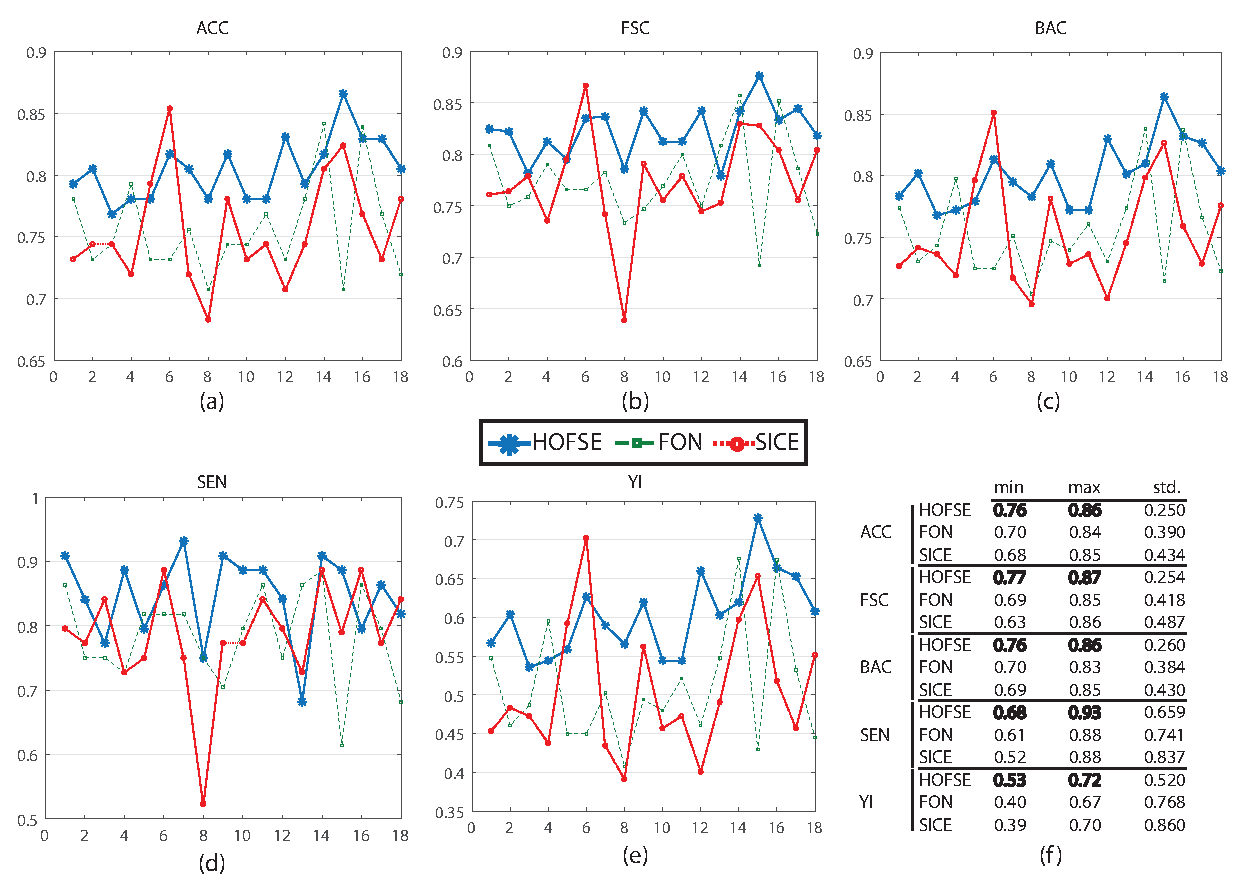
\includegraphics[width=7in]{Final}
		\caption{
			sdsss 
		}
		\label{g3.2}
	\end{figure*}
	
	
	Figure \eqref{g3.2} shows the performance of these three methods in all five measurements. Some statistical information about these plots are also included in the embedded table. As it can bee seen in this figure, similar to the accuracy, the proposed method in overall works much better than FON and k-SICE. For a better Demonstration, table \eqref{AVG} provides the average of several classification measurements scores for all permutations. 
	\begin{table}
		\begin{center}
			\caption{The Average of Different Classification Measurements in all perturbations in \% }
			%\resizebox{\textwidth}{!}{  
			\begin{tabular}{@{}c*{6}{c}}
				\hline\hline
				Method&ACC& F-Score&SEN & SPE &YI & BAC 
				\\
				\hline
				k-SICE  &75.57& 77.36 & 78.50 & 72.19 & 50.69 & 75.34 
				\\
				FON   &75.66& 77.44 & 78.40 & 72.48 & 50.89 & 75.44  
				\\
				TBNA &\textbf{80.43}& \textbf{82.20} & \textbf{84.60} & \textbf{75.59} & \textbf{60.20} & \textbf{80.09}
				
				\\
				
				\hline\hline
				\label{AVG}
			\end{tabular}
			%}
		\end{center}
	\end{table}
	As it can be seen in this table, the average accuracy of TBNA which is $80.43 \%$ is $4.77\%$ higher than the next method HON, and $4.86 \%$ better than k-SICE. It is noteworthy that The other two methods i.e HON and SICE shows similar results in average.  
	
	\begin{figure*}
		\centering
		
\includegraphics[width=7in]{FG}
		\caption{
			The difference graph. This graph is obtained via subtracting the functional connectivity of eMCI subjects from normal subjects. Each circle represents a ROI in AAL atlas and the color and size of each circle is proportional to the graph clustering coefficient of the difference graph. red = more activity in EMCI, green: less. 
		}
		\label{g3.3}
	\end{figure*}
	
	\subsubsection{Runtime Comparison}
	One other key features of TBNA is that it works significantly faster that the other two methods. Table \eqref{Time} shows the average elapsed time (Training plus Testing) of each method for all selected permutations. These methods were executed in matlab R2017b and carried with an intel Core-i7 processor and $16$GB of RAM. As it can be seen in this table, TBNA is more that $600$ times faster than HON and $20$ times faster that SICE.   
	\begin{table}
		\begin{center}
			\caption{Elapsed time of the test and train phase in seconds}
			%\resizebox{\textwidth}{!}{  
			\begin{tabular}{@{}c*{4}{c}}
				\hline\hline
				Method& HON & k-SICE& TBNA  
				\\
				\hline
				Elapsed Time  &6950& 230 & 11 
				\\
				\hline\hline
				\label{Time}
			\end{tabular}
			%}
		\end{center}
	\end{table}
	Having a huge execution time specially affects the parameter selection for HON, since it uses cross-validation procedure in order to find the optimal parameters which itself require several  runs of the algorithm. 
	
	%\subsubsection{Parameter Estimation and Sensitivity}
	%As it was discussed before, the choice of parameters drastically affect the performance of the aforementioned classifier. 
	
	
	
	\subsection{Functional connectivity Network}
	The functional connectivity networks of the Normal and eMCI classes was obtained via TBNA as it is described in \eqref{FC_Construction}.
	In order to better highlight the differences between Normal and eMCI subjects, a difference graph $D$ is constructed by subtracting the Normal FC from the eMCI FC. This graph could be seen in Figure\eqref{g3.3}. 
	The nodes of $D$ shows the ROIs according to the AAL atlas. The size of each node is proportional to its graph clustering coefficient, i.e. the bigger node, demonstrates higher activity in eMCI subjects in the corresponding ROI. 
	Similar to nodes, the size of each edge is also proportional to the correlation between two ROI's. In addition, the edges are also color coded in a way that the green edges shows the positive edges in $D$ and the orange edges shows the negative edges in $D$. In this manner, the green edges demonstrates decreasing in activity between the corresponding nodes in eMCI subjects and vice versa, the orange edges shows increasing activity between corresponding ROIs in the eMCI subjects.   
	
	As it can be seen in the difference graph, the big nodes i.e. ROIs with higher activities does not necessarily establish strong connections with the other nodes. As an obvious example, higher activities in Lingual gyrus(ROI index: 47,48)\cite{r24,r25}, Calcarine sulcus(ROI index: 43, 44)\cite{r26,r27}, Supplementary motor area(ROI index: 19,20)\cite{r27,r28} and Temporal\_mid\_L(ROI index: 85)\cite{r29} are easily detectable. The majority of ROIs located in frontal lobe also shows rather high activities comparing to normal subjects\cite{r31,r30}.
	
	Similar to the nodes, strong edge between two ROIs does not necessarily requires the nodes to be highly active in eMCI. Although a strong edge does indicate high activities and functional connectivity between the two corresponding ROIs. The difference Graph shows significant increase in connectivity between 
	Rectus(ROI index: 28, 27 in Frontal lobe) and 
	Parietal\_Sup\_R(ROI index: 60 in Parietal lobe),
	Frontal\_Inf\_Orb\_R(ROI index: 16 in Frontal lobe) and
	Cingulum\_Ant(ROI index: 31,32 in Limbic lobe), 
	Insula\_L, Temporal\_Pole\_Sup\_L(ROI index: 29,83 in Limbic lobe) and
	Pallidum\_R, Caudate\_R(ROI index: 29,83 in Sub Cortical Grey Nuclei). It can also be seen that within activities in frontal lobe also increased in patients with eMCI. There is a decrease in connectivity between Amygdala\_L(ROI index: 41 in Sub Cortical Grey Nuclei) with Frontal\_Mid\_Orb\_R(ROI index: 10 in Sub Frontal lobe) and ParaHippocampal\_L(ROI index: 39 in Sub Limbic lobe). The connectivity between Heschl\_L(ROI index: 79 in Temporal lobe) and two ROIs Temporal\_Mid\_R(ROI index: 86 also in Temporal lobe) and Occipital\_Inf\_R(ROI index: 54 in Occipital lobe) also decreased in eMCI.  
	
	\subsubsection*{Regarding the Cerebellum and Vermis}
	In fMRI data analysis and especially in Alzheimer's disease studies, ROIs within the Cerebellum and Vermis are usually excluded[ref] since their role was regarded as insignificant. Recent studies have shown that the traditional assumption that Cerebral area is essential only for the coordination of voluntary motor activity and motor learning is not valid and indicates the significant role of cerebellum in nervous system function, cognition and emotion\cite{r32}. 
	
	As it can be seen in the difference graph that we obtained, ROIs within Cerebellum and Vermis are highly active and both their intra and inter connections are noticeable. There is an increasing functional connectivity between the Limbic lobe especially 
	Hippocampus\_R, Temporal\_Pole\_Mid(ROI index: 38,87,88)
	and Cerebral areas in eMCI patients. Also, the connectivity between Occipital lobe, especially Occipital\_mid\_R(ROI index: 52), the Frontal lobe, especially in Frontal\_mid\_orb(ROI index: 9,10) and Cerebral areas seems to decrease in patients with eMCI.
	
	
	
	
	%\begin{table*}
	%	\begin{center}
	%		\caption{Active Nodes }
	%		\resizebox{\textwidth}{!}{  
	%		\begin{tabular}{@{}l*{4}{l}}
	%			\hline\hline
	%			NO.&ROI Index&ROI name&Location& Citations 
	%			\\
	%			\hline
	%			1& 8 & Frontal\_Mid\_R & Middle frontal gyrus
	%			$\rightarrow$ Prefrontal cortex $\rightarrow$ \textbf{Frontal lobe}
	%			 & Main 
	%			\\
	%			2& 14 & Frontal\_Inf\_Tri\_R & Inferior frontal gyrus, pars triangularis
	%			$\rightarrow$ Inferior frontal gyrus $\rightarrow$ Prefrontal cortex
	%			 $\rightarrow$ \textbf{Frontal lobe} & Main 
	%			\\
	%			3& 17 & Rolandic\_Oper\_L & Rolandic operculum
	%			$\rightarrow$ Operculum $\rightarrow$ \textbf{Cerebral cortex} & Main 
	%			\\
	%			4& 19 & Supp\_Motor\_Area\_L & Supplementary motor area
	%			$\rightarrow$ Motor area $\rightarrow$ \textbf{Functional area} & Main 
	%			\\
	%			5& 20 & Supp\_Motor\_Area\_R & Supplementary motor area
	%			$\rightarrow$ Motor area $\rightarrow$ \textbf{Functional area} & Main 
	%			\\
	%			6& 25 & Frontal\_Med\_Orb\_L &  Medial orbitofrontal cortex $\rightarrow$ Orbitofrontal cortex
	%			$\rightarrow$ Orbitofrontal area $\rightarrow$ \textbf{Frontal lobe} & ? 
	%			\\
	%			7 & 34 & Cingulum\_Mid\_R & Right midcingulate area
	%			$\rightarrow$ Midcingulate area $\rightarrow$ Cingulate gyrus
	%			$\rightarrow$ Cerebral cortex $\rightarrow$ \textbf{Frontal lobe} & ? 
	%			\\
	%			8 & 43 & Calcarine\_L & Calcarine sulcus
	%			$\rightarrow$ Midcingulate area $\rightarrow$ \textbf{Sulcus} & ? 
	%			\\
	%			9 & 44 & Calcarine\_R & Calcarine sulcus
	%			$\rightarrow$ Midcingulate area $\rightarrow$ \textbf{Sulcus} & ? 
	%			\\
	%			10 & 47 & Lingual\_L & Lingual gyrus
	%			$\rightarrow$ Occipital lobe $\rightarrow$Cerebral cortex $\rightarrow$ \textbf{Frontal lobe} & ? 
	%			\\
	%			11 & 48 & Lingual\_R & Lingual gyrus
	%			$\rightarrow$ Occipital lobe $\rightarrow$Cerebral cortex $\rightarrow$ \textbf{Frontal lobe} & ? 
	%			\\
	%			12 & 70 & Paracentral\_Lobule\_R & Paracentral lobule $\rightarrow$ \textbf{Frontal lobe} & ?
	%			\\
	%			13 & 69 & Paracentral\_Lobule\_L & Middle temporal gyrus $\rightarrow$ \textbf{Temporal lobe} & ?
	%			\\
	%			14 & 99 & Cerebelum\_6\_L & Lobule VI of cerebellar hemisphere $\rightarrow$Cerebellum
	%			$\rightarrow$ Metencephalon $\rightarrow$ \textbf{Hindbrain} & ?
	%			\\
	%			15 & 111 & Vermis\_4\_5 & Vermis $\rightarrow$ Cerebellum $\rightarrow$ Metencephalon $\rightarrow$ \textbf{Hindbrain} & ?
	%			\\
	%			\hline\hline
	%			\label{sss}
	%		\end{tabular}
	%		}
	%	\end{center}
	%\end{table*}
	
	
	
	
	% An example of a floating figure using the graphicx package.
	% Note that \label must occur AFTER (or within) \caption.
	% For figures, \caption should occur after the \includegraphics.
	% Note that IEEEtran v1.7 and later has special internal code that
	% is designed to preserve the operation of \label within \caption
	% even when the captionsoff option is in effect. However, because
	% of issues like this, it may be the safest practice to put all your
	% \label just after \caption rather than within \caption{}.
	%
	% Reminder: the "draftcls" or "draftclsnofoot", not "draft", class
	% option should be used if it is desired that the figures are to be
	% displayed while in draft mode.
	%
	%\begin{figure}[!t]
	%\centering
	%\includegraphics[width=2.5in]{myfigure}
	% where an .eps filename suffix will be assumed under latex, 
	% and a .pdf suffix will be assumed for pdflatex; or what has been declared
	% via \DeclareGraphicsExtensions.
	%\caption{Simulation results for the network.}
	%\label{fig_sim}
	%\end{figure}
	
	% Note that the IEEE typically puts floats only at the top, even when this
	% results in a large percentage of a column being occupied by floats.
	
	
	% An example of a double column floating figure using two subfigures.
	% (The subfig.sty package must be loaded for this to work.)
	% The subfigure \label commands are set within each subfloat command,
	% and the \label for the overall figure must come after \caption.
	% \hfil is used as a separator to get equal spacing.
	% Watch out that the combined width of all the subfigures on a 
	% line do not exceed the text width or a line break will occur.
	%
	%\begin{figure*}[!t]
	%\centering
	%\subfloat[Case I]{\includegraphics[width=2.5in]{box}%
	%\label{fig_first_case}}
	%\hfil
	%\subfloat[Case II]{\includegraphics[width=2.5in]{box}%
	%\label{fig_second_case}}
	%\caption{Simulation results for the network.}
	%\label{fig_sim}
	%\end{figure*}
	%
	% Note that often IEEE papers with subfigures do not employ subfigure
	% captions (using the optional argument to \subfloat[]), but instead will
	% reference/describe all of them (a), (b), etc., within the main caption.
	% Be aware that for subfig.sty to generate the (a), (b), etc., subfigure
	% labels, the optional argument to \subfloat must be present. If a
	% subcaption is not desired, just leave its contents blank,
	% e.g., \subfloat[].
	
	
	% An example of a floating table. Note that, for IEEE style tables, the
	% \caption command should come BEFORE the table and, given that table
	% captions serve much like titles, are usually capitalized except for words
	% such as a, an, and, as, at, but, by, for, in, nor, of, on, or, the, to
	% and up, which are usually not capitalized unless they are the first or
	% last word of the caption. Table text will default to \footnotesize as
	% the IEEE normally uses this smaller font for tables.
	% The \label must come after \caption as always.
	%
	%\begin{table}[!t]
	%% increase table row spacing, adjust to taste
	%\renewcommand{\arraystretch}{1.3}
	% if using array.sty, it might be a good idea to tweak the value of
	% \extrarowheight as needed to properly center the text within the cells
	
	\
	
	
	
	
	
	
	
	
	
	
	
	
	
	
	
	
	
	
	
	
	
	
	%\caption{An Example of a Table}
	%\label{table_example}
	%\centering
	%% Some packages, such as MDW tools, offer better commands for making tables
	%% than the plain LaTeX2e tabular which is used here.
	%\begin{tabular}{|c||c|}
	%\hline
	%One & Two\\
	%\hline
	%Three & Four\\
	%\hline
	%\end{tabular}
	%\end{table}
	
	
	% Note that the IEEE does not put floats in the very first column
	% - or typically anywhere on the first page for that matter. Also,
	% in-text middle ("here") positioning is typically not used, but it
	% is allowed and encouraged for Computer Society conferences (but
	% not Computer Society journals). Most IEEE journals/conferences use
	% top floats exclusively. 
	% Note that, LaTeX2e, unlike IEEE journals/conferences, places
	% footnotes above bottom floats. This can be corrected via the
	% \fnbelowfloat command of the stfloats package.
	
	
	
	
	\section{Conclusion}
	The majority of classification techniques uses the vectorized version of data as the input of the discriminant function. As the number of the dimensions grows, i.e. when data is naturally a high order tensor, this vectorization become problematic and it would highly affect the  performance. Taking advantage of the techniques designed for the tensors, we have developed a framework for fMRI data analysis in which the following objectives: 
	\begin{enumerate}
		\item 
		Dimension Reduction
		\item 
		Classification 
		\item 
		Obtaining Functional Connectivity networn 
	\end{enumerate}
	are achieved via a singe \textbf{H}igh \textbf{O}rder \textbf{SVD} of the input tensors. 
	
	Extensive studies on the rs-fMRI provided by ADNI shows the superiority of the proposed framework in both classification and functional connectivity. The obtained FC network not only acknowledge the previous discovered connections but also reveals new connectivity patterns previously unknown.
	The framework proposed in this paper can be easily extended to other studies involved with high order data.  
	
	%\begin{table*}
	%	\begin{center}
	%		\caption{content...}
	%		\resizebox{\textwidth}{!}{  
	%	\begin{tabular}{@{}c*{20}{c}}
	%		\hline\hline
	%		\multicolumn{20}{c}{Datasets} 
	%		\\
	%		\hline
	%&\multicolumn{1}{|c}{TBNA} & \textbf{79.27} & \textbf{80.49} & \textbf{76.83} & 78.05 & 78.05 & 81.71 & \textbf{80.49} & \textbf{78.05} & \textbf{81.71} & \textbf{78.05} & \textbf{78.05} & \textbf{83.1} & \textbf{79.27} & 8171 & \textbf{86.59} & 82.93 & \textbf{82.93} & \textbf{80.49} 
	%\\
	%ACC&\multicolumn{1}{|c}{FON} & 78.05 & 73.17 & 74.39 & \textbf{79.27} & 73.17 & 73.17 & 75.61 & 70.73 & 74.39 & 74.39 & 76.83 & 73.17 & 78.05 & \textbf{84.15} & 70.73 & \textbf{83.9} & 76.83 & 71.95 
	%\\
	%&\multicolumn{1}{|c}{SICE} & 73.17 & 74.39 & 74.39 & 71.95 & \textbf{79.27} & \textbf{85.37} & 71.95 & 68.29 & 78.05 & 73.17 & 74.39 & 70.73 & 74.39 & 80.49 & 82.38 & 76.83 & 73.17 & 78.05 
	%%\\\hline
	%%&\multicolumn{1}{|c}{TBNA} & \textbf{0.9091} & \textbf{0.8409} & 0.7727 & \textbf{0.8864} & 0.7955 & \textbf{0.8636} & \textbf{0.9318} & 0.75 & \textbf{0.9091} & \textbf{0.8864} & \textbf{0.8864} & \textbf{0.8421} & 0.6818 & \textbf{0.9091} & \textbf{0.8864} &\textbf{ 0.7955} &\textbf{ 0.8636} & \textbf{0.8182} 
	%%\\
	%%SEN&\multicolumn{1}{|c}{FON} & 0.8636 & 0.75 & 0.75 & 0.7273 & \textbf{0.8182} & 0.8182 & 0.8182 & 0.75 & 0.7045 & 0.7955 & 0.8636 & 0.75 & \textbf{0.8636} & 0.8864 & 0.6136 & 0.8636 & 0.7955 & 0.6818 
	%%\\
	%%&\multicolumn{1}{|c}{SICE} & 0.7955 & 0.7727 & \textbf{0.8409} & 0.7273 & 0.75 & 0.8864 & 0.75 & 0.5227 & 0.7727 & 0.7727 & 0.8409 & 0.7955 & 0.7273 & 0.8864 & 0.7895 & 0.8864 & 0.7727 & 0.8409 
	%\\\hline
	%%&\multicolumn{1}{|c}{TBNA} & 0.6579 & \textbf{0.7632} & \textbf{0.7632} & 0.6579 & \textbf{0.7632} & 0.7632 & 0.6579 & 0.8158 & 0.7105 & 0.6579 & 0.6579 & 0.8182 & 0.9211 & 0.7105 & 0.8421 & 0.8684 & 0.7895 & 0.7895 
	%%\\
	%%SPE&\multicolumn{1}{|c}{FON} & 0.6842 & 0.7105 & 0.7368 & 0.8684 & 0.6316 & 0.6316 & 0.6842 & 0.6579 & 0.7895 & 0.6842 & 0.6579 & 0.7105 & 0.6842 & 0.7895 & 0.8158 & 0.8106 & 0.7368 & 0.7632 
	%%\\
	%%&\multicolumn{1}{|c}{SICE} & 0.6579 & 0.7105 & 0.6316 & 0.7105 & 0.8421 & 0.8158 & 0.6842 & 0.8684 & 0.7895 & 0.6842 & 0.6316 & 0.6053 & 0.7632 & 0.7105 & 0.8636 & 0.6316 & 0.6842 & 0.7105 
	%%\\\hline
	%%&\multicolumn{1}{|c}{TBNA} & 0.567 & 0.6041 & 0.5359 & 0.5443 & 0.5586 & 0.6268 & 0.5897 & 0.5658 & 0.6196 & 0.5443 & 0.5443 & 0.6603 & 0.6029 & 0.6196 & 0.7285 & 0.6639 & 0.6531 & 0.6077 
	%%\\
	%%YI&\multicolumn{1}{|c}{FON} & 0.5478 & 0.4605 & 0.4868 & 0.5957 & 0.4498 & 0.4498 & 0.5024 & 0.4079 & 0.494 & 0.4797 & 0.5215 & 0.4605 & 0.5478 & 0.6758 & 0.4294 & 0.6742 & 0.5323 & 0.445 
	%%\\
	%%&\multicolumn{1}{|c}{SICE} & 0.4533 & 0.4833 & 0.4725 & 0.4378 & 0.5921 & 0.7022 & 0.4342 & 0.3911 & 0.5622 & 0.4569 & 0.4725 & 0.4007 & 0.4904 & 0.5969 & 0.6531 & 0.5179 & 0.4569 & 0.5514 
	%%\\\hline
	%&\multicolumn{1}{|c}{TBNA} &\textbf{ 82.47} & \textbf{82.22} & \textbf{78.16} & \textbf{81.25} & \textbf{79.55} & 83.52 & \textbf{83.67} &\textbf{ 78.57} & \textbf{84.21} & \textbf{81.25 } & \textbf{81.25} & \textbf{84.25} & 77.92 & 84.21 & \textbf{87.64 }& 83.33 & \textbf{84.44} & \textbf{81.82 }
	%\\
	%F-SC&\multicolumn{1}{|c}{FON} & 80.85 & 75 & 75.86 & 79.01 & 76.6 & 76.6 & 78.26 & 73.33 & 74.7 & 76.92 & 80 & 75 & \textbf{80.85} & \textbf{85.71} & 69.23 & \textbf{85.2} & 78.65 & 72.29 
	%\\
	%&\multicolumn{1}{|c}{SICE} & 76.09 & 76.4 & 77.89 & 73.56 & 79.52 & \textbf{86.67} & 74.16 & 63.89 & 79.07 & 75.56 & 77.89 & 74.47 & 75.29 & 82.98 & 82.79 & 80.41 & 75.56 & 80.43 
	%\\\hline
	%%&\multicolumn{1}{|c}{TBNA} & 0.7835 & 0.802 & 0.7679 & 0.7721 & 0.7793 & 0.8134 & 0.7949 & 0.7829 & 0.8098 & 0.7721 & 0.7721 & 0.8301 & 0.8014 & 0.8098 & 0.8642 & 0.8319 & 0.8266 & 0.8038 
	%%\\
	%%BAC&\multicolumn{1}{|c}{FON} & 0.7739 & 0.7303 & 0.7434 & 0.7978 & 0.7249 & 0.7249 & 0.7512 & 0.7039 & 0.747 & 0.7398 & 0.7608 & 0.7303 & 0.7739 & 0.8379 & 0.7147 & 0.8371 & 0.7661 & 0.7225 
	%%\\
	%%&\multicolumn{1}{|c}{SICE} & 0.7267 & 0.7416 & 0.7362 & 0.7189 & 0.7961 & 0.8511 & 0.7171 & 0.6956 & 0.7811 & 0.7285 & 0.7362 & 0.7004 & 0.7452 & 0.7984 & 0.8266 & 0.759 & 0.7285 & 0.7757 
	%%		& HON & &\multicolumn{1}{|c}{kernel} & \\
	%%		
	%%		& TBNA & &\multicolumn{1}{|c}{kernel} & \\
	%		 \\
	%		\hline\hline
	%	\end{tabular}
	%}
	%	\end{center}
	%\end{table*}
	
	
	
	
	
	
	
	% if have a single appendix:
	%\appendix[Proof of the Zonklar Equations]
	% or
	%\appendix  % for no appendix heading
	% do not use \section anymore after \appendix, only \section*
	% is possibly needed
	
	% use appendices with more than one appendix
	% then use \section to start each appendix
	% you must declare a \section before using any
	% \subsection or using \label (\appendices by itself
	% starts a section numbered zero.)
	%
	
	
	%\appendices
	%\section{Proof of the First Zonklar Equation}
	%Appendix one text goes here.
	
	% you can choose not to have a title for an appendix
	% if you want by leaving the argument blank
	%\section{}
	%Appendix two text goes here.
	
	
	% use section* for acknowledgment
	\section*{Acknowledgment}
	
	
	The authors would like to thank...
	
	
	% Can use something like this to put references on a page
	% by themselves when using endfloat and the captionsoff option.
	\ifCLASSOPTIONcaptionsoff
	\newpage
	\fi
	
	
	
	% trigger a \newpage just before the given reference
	% number - used to balance the columns on the last page
	% adjust value as needed - may need to be readjusted if
	% the document is modified later
	%\IEEEtriggeratref{8}
	% The "triggered" command can be changed if desired:
	%\IEEEtriggercmd{\enlargethispage{-5in}}
	
	% references section
	
	% can use a bibliography generated by BibTeX as a .bbl file
	% BibTeX documentation can be easily obtained at:
	% http://mirror.ctan.org/biblio/bibtex/contrib/doc/
	% The IEEEtran BibTeX style support page is at:
	% http://www.michaelshell.org/tex/ieeetran/bibtex/
	%\bibliographystyle{IEEEtran}
	% argument is your BibTeX string definitions and bibliography database(s)
	%\bibliography{IEEEabrv,../bib/paper}
	%
	% <OR> manually copy in the resultant .bbl file
	% set second argument of \begin to the number of references
	% (used to reserve space for the reference number labels box)
	\begin{thebibliography}{1}
		
		\bibitem{r01}
		Caselli, Richard J., et al. "Longitudinal changes in cognition and behavior in asymptomatic carriers of the APOE e4 allele." Neurology 62.11 (2004): 1990-1995.
		
		\bibitem{r02}
		Brookmeyer, Ron, et al. "Forecasting the global burden of Alzheimer’s disease." Alzheimer's \& dementia: the journal of the Alzheimer's Association 3.3 (2007): 186-191.
		
		\bibitem{r03}
		Musha, Toshimitsu, et al. "EEG markers for characterizing anomalous activities of cerebral neurons in NAT (neuronal activity topography) method." IEEE Transactions on Biomedical Engineering 60.8 (2013): 2332-2338.
		
		\bibitem{r04}
		Gould, R. L., et al. "Brain mechanisms of successful compensation during learning in Alzheimer disease." Neurology 67.6 (2006): 1011-1017.
		
		\bibitem{r05}
		Richiardi, Jonas, et al. "Classifying minimally disabled multiple sclerosis patients from resting state functional connectivity." Neuroimage 62.3 (2012): 2021-2033.
		
		\bibitem{r06}
		Yang, Xue, et al. "Evaluation of statistical inference on empirical resting state fMRI." IEEE Transactions on Biomedical Engineering 61.4 (2014): 1091-1099.
		
		\bibitem{r07}
		R. Graaf and K. Kevin. Methods and apparatus for
		compensating eld inhomogeneities in magnetic resonance
		studies. US Patent No. 8035387, 2011.
		
		\bibitem{r08}
		Zhang, Xiaowei, et al. "Resting-state whole-brain functional connectivity networks for mci classification using l2-regularized logistic regression." IEEE transactions on nanobioscience 14.2 (2015): 237-247.
		
		\bibitem{r09}
		Stanley, Matthew Lawrence, et al. "Defining nodes in complex brain networks." Frontiers in computational neuroscience 7 (2013): 169.
		
		\bibitem{r10}
		Jie, Biao, et al. "Integration of network topological and connectivity properties for neuroimaging classification." IEEE transactions on biomedical engineering 61.2 (2014): 576-589.
		
		\bibitem{r11}
		Wee, Chong-Yaw, et al. "Resting-state multi-spectrum functional connectivity networks for identification of MCI patients." PloS one 7.5 (2012): e37828.
		
		\bibitem{r12}
		Tibshirani, Robert, et al. "Sparsity and smoothness via the fused lasso." Journal of the Royal Statistical Society: Series B (Statistical Methodology) 67.1 (2005): 91-108.
		
		\bibitem{r13}
		Wright, John, et al. "Robust face recognition via sparse representation." IEEE transactions on pattern analysis and machine intelligence 31.2 (2009): 210-227.
		
		\bibitem{r14}
		Zhang, Jianjia, et al. "Functional brain network classification with compact representation of SICE matrices." IEEE Transactions on Biomedical Engineering 62.6 (2015): 1623-1634.
		
		\bibitem{r15}
		Huang, Shuai, et al. "Learning brain connectivity of Alzheimer's disease by sparse inverse covariance estimation." NeuroImage 50.3 (2010): 935-949.
		
		\bibitem{r16}
		Allen, Elena A., et al. "Tracking whole-brain connectivity dynamics in the resting state." Cerebral cortex 24.3 (2014): 663-676.
		
		\bibitem{r17}
		Damaraju, Eswar, et al. "Dynamic functional connectivity analysis reveals transient states of dysconnectivity in schizophrenia." NeuroImage: Clinical 5 (2014): 298-308.
		
		\bibitem{r18}
		Hutchison, R. Matthew, et al. "Dynamic functional connectivity: promise, issues, and interpretations." Neuroimage 80 (2013): 360-378.
		
		\bibitem{r19}
		Leonardi, Nora, et al. "Principal components of functional connectivity: a new approach to study dynamic brain connectivity during rest." NeuroImage 83 (2013): 937-950.
		
		\bibitem{r20}
		Leonardi, Nora, et al. "Principal components of functional connectivity: a new approach to study dynamic brain connectivity during rest." NeuroImage 83 (2013): 937-950.
		
		\bibitem{r21}
		Nordberg, Agneta. "PET imaging of amyloid in Alzheimer's disease." The lancet neurology 3.9 (2004): 519-527.
		
		\bibitem{r22}
		Jeong, Jaeseung. "EEG dynamics in patients with Alzheimer's disease." Clinical neurophysiology 115.7 (2004): 1490-1505.
		
		\bibitem{r23}
		Jeong, Jaeseung. "EEG dynamics in patients with Alzheimer's disease." Clinical neurophysiology 115.7 (2004): 1490-1505.
		
		\bibitem{r24}Golby, Alexandra, et al. "Memory encoding in Alzheimer's disease: an fMRI study of explicit and implicit memory." Brain 128.4 (2005): 773-787.
		
		\bibitem{r25}He, Yong, et al. "Regional coherence changes in the early stages of Alzheimer’s disease: a combined structural and resting-state functional MRI study." Neuroimage 35.2 (2007): 488-500.
		
		
		
		\bibitem{r26}Bakkour, Akram, et al. "The effects of aging and Alzheimer's disease on cerebral cortical anatomy: specificity and differential relationships with cognition." Neuroimage 76 (2013): 332-344.
		
		\bibitem{r27}Brewer, Alyssa A., and Brian Barton. "Visual cortex in aging and Alzheimer's disease: changes in visual field maps and population receptive fields." Frontiers in psychology 5 (2014): 74.
		
		\bibitem{r28}Jacobsen, Jörn-Henrik, et al. "Why musical memory can be preserved in advanced Alzheimer’s disease." Brain 138.8 (2015): 2438-2450.
		
		\bibitem{r29}Kosicek, Marko, and Silva Hecimovic. "Phospholipids and Alzheimer’s disease: alterations, mechanisms and potential biomarkers." International journal of molecular sciences 14.1 (2013): 1310-1322.
		
		\bibitem{r30}Salvatore, Christian, et al. "Magnetic resonance imaging biomarkers for the early diagnosis of Alzheimer's disease: a machine learning approach." Frontiers in neuroscience 9 (2015): 307.
		
		\bibitem{r31}Gould, R. L., et al. "Brain mechanisms of successful compensation during learning in Alzheimer disease." Neurology 67.6 (2006): 1011-1017.
		
		\bibitem{r32}Jacobs, Heidi IL, et al. "The cerebellum in Alzheimer’s disease: evaluating its role in cognitive decline." Brain 141.1 (2017): 37-47.
		
		\bibitem{r33}
		\bibitem{r34}
		\bibitem{r35}
		
		
	\end{thebibliography}
	
	% biography section
	% 
	% If you have an EPS/PDF photo (graphicx package needed) extra braces are
	% needed around the contents of the optional argument to biography to prevent
	% the LaTeX parser from getting confused when it sees the complicated
	% \includegraphics command within an optional argument. (You could create
	% your own custom macro containing the \includegraphics command to make things
	% simpler here.)
	%\begin{IEEEbiography}[{\includegraphics[width=1in,height=1.25in,clip,keepaspectratio]{mshell}}]{Michael Shell}
	% or if you just want to reserve a space for a photo:
	
	\begin{IEEEbiography}{Ali Noroozi}
		
	\end{IEEEbiography}
	
	% if you will not have a photo at all:
	\begin{IEEEbiographynophoto}{Mansoor Rezghi}
		
	\end{IEEEbiographynophoto}
	
	% insert where needed to balance the two columns on the last page with
	% biographies
	%\newpage
	
	%\begin{IEEEbiographynophoto}{Mansoor Rezghi}
	%Biography text here.
	%\end{IEEEbiographynophoto}
	
	% You can push biographies down or up by placing
	% a \vfill before or after them. The appropriate
	% use of \vfill depends on what kind of text is
	% on the last page and whether or not the columns
	% are being equalized.
	
	%\vfill
	
	% Can be used to pull up biographies so that the bottom of the last one
	% is flush with the other column.
	%\enlargethispage{-5in}
	
	
	
	% that's all folks
\end{document}







% The feature extraction methods are: \textbf{Naive Vectorization(NV):} which is the vectorized raw samples, \textbf{SICE Vectorized(SICE-V):} the vectorization of SICE matrices, \textbf{TBNA Vectorized(TBNA-V):} the vectorization of TBNA matrices, \textbf{SLR Vectorized(SLR-V):} the vectorization of SLR matrices, \textbf{SICE} and \textbf{TBNA} 